% !TEX encoding = ITF-8 Unicode
%
% Niniejszy plik stanowi przykład formatowania pracy magisterskiej na
% Wydziale MIM UW.  Szkielet użytych poleceń można wykorzystywać do
% woli, np. formatujac wlasna prace.
%
% Zawartosc merytoryczna stanowi oryginalnosiagniecie
% naukowosciowe Marcina Wolinskiego.  Wszelkie prawa zastrzeżone.
%
% Copyright (c) 2001 by Marcin Woliński <M.Wolinski@gust.org.pl>
% Poprawki spowodowane zmianami przepisów - Marcin Szczuka, 1.10.2004
% Poprawki spowodowane zmianami przepisow i ujednolicenie 
% - Seweryn Karłowicz, 05.05.2006
% dodaj opcję [licencjacka] dla pracy licencjackiej
\documentclass{pracamgr}

\usepackage{polski}

%Jesli uzywasz kodowania polskich znakow ISO-8859-2 nastepna linia powinna byc 
%odkomentowana
%\usepackage[latin2]{inputenc}
%Jesli uzywasz kodowania polskich znakow CP-1250 to ta linia powinna byc 
%odkomentowana
\usepackage[utf8]{inputenc}
\RequirePackage{graphicx}
\usepackage{wrapfig}
\RequirePackage{longtable}
\usepackage[usenames,dvipsnames]{color}
\usepackage{subfigure}
%\usepackage{hyperref}
%\usepackage{url}
\definecolor{gray}{RGB}{50,50,50}
\usepackage[toc,page]{appendix}
\renewcommand{\appendixtocname}{Dodatki} 
% \renewcommand{\appendixpage}{\part*{Dodatki}}

\usepackage[colorlinks=true,linkcolor=gray,urlcolor=blue]{hyperref}  



\newcommand{\emptyP}{\mbox{$\epsilon$}}
\newcommand{\terminal}[1]{\mbox{{\texttt {#1}}}}
\newcommand{\nonterminal}[1]{\mbox{$\langle \mbox{{\sl #1 }} \! \rangle$}}
\newcommand{\arrow}{\mbox{::=}}
\newcommand{\delimit}{\mbox{$|$}}
\newcommand{\reserved}[1]{\mbox{{\texttt {#1}}}}
\newcommand{\literal}[1]{\mbox{{\texttt {#1}}}}
\newcommand{\symb}[1]{\mbox{{\texttt {#1}}}}
% Dane magistranta:

\author{Imię i nazwisko}

\nralbumu{nralbumu}

\title{Intuicyjny język wyszukiwania TQL (Tablets Query Language)}

\tytulang{Intuitive query language TQL (Tablets Query Language)}

%kierunek: Matematyka, Informatyka, ...
\kierunek{Informatyka}

% informatyka - nie okreslamy zakresu (opcja zakomentowana)
% matematyka - zakres moze pozostac nieokreslony,
% a jesli ma byc okreslony dla pracy mgr,
% to przyjmuje jedna z wartosci:
% {metod matematycznych w finansach}
% {metod matematycznych w ubezpieczeniach}
% {matematyki stosowanej}
% {nauczania matematyki}
% Dla pracy licencjackiej mamy natomiast
% mozliwosc wpisania takiej wartosci zakresu:
% {Jednoczesnych Studiow Ekonomiczno--Matematycznych}

% \zakres{Tu wpisac, jesli trzeba, jedna z opcji podanych wyzej}

% Praca wykonana pod kierunkiem:
% (podać tytuł/stopień imię i nazwisko opiekuna
% Instytut
% ew. Wydział ew. Uczelnia (jeżeli nie MIM UW))
\opiekun{dra Roberta Dąbrowskiego\\
  Instytut Informatyki\\
  }

% miesiąc i~rok:
\date{czerwiec 2010}

%Podać dziedzinę wg klasyfikacji Socrates-Erasmus:
\dziedzina{ 
%11.0 Matematyka, Informatyka:\\ 
%11.1 Matematyka\\ 
%11.2 Statystyka\\ 
11.3 Informatyka\\ 
%11.4 Sztuczna inteligencja\\ 
%11.5 Nauki aktuarialne\\
%11.9 Inne nauki matematyczne i informatyczne
}

%Klasyfikacja tematyczna wedlug AMS (matematyka) lub ACM (informatyka)
\klasyfikacja{H. INFORMATION SYSTEMS\\
H.2. DATABASE MANAGEMENT\\
H.2.3 Languages}

% Słowa kluczowe:
\keywords{tabliczka, sumerologia, kliny, odczyty, język dziedzinowy, DSL, Domain-Specific Languages}

% Tu jest dobre miejsce na Twoje własne makra i~środowiska:
\newtheorem{defi}{Definicja}[section]

% koniec definicji

\begin{document}
\maketitle

%tu idzie streszczenie na strone poczatkowa
\begin{abstract}
Sumerologia jest dziedziną badań nad antycznym językiem Sumerów, w której
kluczowym zagadnieniem jest przeszukiwanie dużych zbiorów informacji
zapisanych na odnalezionych tabliczkach sumeryjskich.


%TODO: przeformułować - powtórzenia
W pracy przedstawiono definicję przeznaczonego dla sumerologów intuicyjnego
języka przeszukiwania zbiorów tabliczek (Tablets Query Language) wraz z jego
przykładowymi implementacjami. Jedna z nich jest oparta na relacyjnej bazie danych, a druga na bazie w postaci pliku XML.

Celem tej pracy jest stworzenie języka zapytań intuicyjnego dla sumerologów,
stanowiącego znaczące uproszczenie w stosunku do SQL dzięki wprowadzeniu pojęć 
naturalnych dla rozważanej dziedziny. TQL nadal
pozwala na tworzenie skomplikowanych zapytań wyszukujących, natomiast nie 
udostępnia funkcjonalności tworzenia i modyfikowania bazy. Można go rozszerzać 
i zmieniać tak, by mógł służyć do zastosowań z innych dziedzin.
\end{abstract}

\tableofcontents
\chapter*{Wprowadzenie}
\addcontentsline{toc}{chapter}{Wprowadzenie}
% jaka będzie wartość dodana tego co zrobimy
% cała ścieżka Informatyka -> nasza praca
% celem naszym było usystematyzować pracę nad systemami dla sumerologów

% nasza ścieżka: Informatyka -> Inżynieria oprogramowania -> różne podejścia -> domain-specific podejście -> domain specific language
 

% 1. krótki opis problemu - są sumerolodzy, mają tabliczki, chcą sprawnie wyszukiwać
\section*{Opis problemu}
Ok. 3500 lat przed naszą erą starożytni Sumerowie, jako prawdopodobnie pierwsi na świecie, zaczęli używać pisma. 
Ze względu na ksztat liter odciśniętych za pomocą trzciny w miękkiej glinie zostało ono później nazwane pismem klinowym. 
Sumerowie używali go głównie w celach administracyjnych. Zapisywali między innymi rachunki za dostawy zwierząt oraz rozliczenia z 
wykonanej na polu lub w warsztacie pracy i należnej zapłaty. Jednymi z ciekawszych tekstów są tzw. listy królów, na 
których znajdują się daty panowania kolejnych władców i ich osiągnięcia w poszczególnych latach. 
Ważniejsze tabliczki wypalano, jednak większość po pewnym czasie niszczono, aby zużytą glinę można było ponownie wykorzystać. 
Do dzisiaj przetrwały głównie te tabliczki, które zostały wypalone podczas przypadkowego pożaru archiwum. 
Wiele z nich jest zniszczonych, jednak wciąż stanowią ogromną wartość historyczną. 
 
Na podstawie zachowanych tabliczek można się wiele dowiedzieć o historii Sumeru, a także o życiu zwykłych ludzi w tym okresie, 
o ich zarobkach, zasiłkach i dniach wolnych. Odczytywaniem tych informacji zajmują się sumerolodzy z całego świata. 
Aby łatwiej dzielić się zdobytą wiedzą, zaczęli tworzyć cyfrowe bazy tabliczek, dostępne w internecie. 
Największa z nich to Cuneiform Digital Library Initiative (CDLI), zawierająca prawie 225 tys tekstów.

Jednak wyszukiwanie interesujących tabliczek może być w tym momencie uciążliwe. 

Sumerolodzy mogliby skorzystać ze specyficznych dla baz danych języków zapytań (np. SQL), ale po pierwsze większość z 
nich nie zna tych języków, a po drugie budowanie w ten sposób złożonych zapytań dotyczących danych tekstowych jest czasochłonne. 
Takie języki były tworzone z myślą o bardziej generycznych zastosowaniach i nie odpowiadają potrzebom sumerologów.
Z tych powodów większość istniejących obecnie serwisów internetowych udostępnia formularze ułatwiające wprowadzanie kryteriów
 wyszukiwania. Jednak mają one ograniczone możliwości i nie pozwalają na konstruowanie bardziej skomplikowanych zapytań.
Dlatego istnieje potrzeba stworzenia narzędzia wspomagającego wyszukiwanie, które będzie łączyło w sobie jak największą siłę 
wyrazu oraz łatwość użycia dla osób znających jedynie dziedzinę problemu.

% 2. różne podejścia do tworzenia oprogramowania
Przy tego typu problemach z pomocą przychodzi informatyka. 

\section*{Propozycja rozwiązania}
Do tej pory powstało wiele różnych systemów informatycznych, a doświadczenie stopniowo zdobywane przy ich budowie prowadzi do 
ciągłego rozwijania nauki zwanej inżynierią oprogramowania, zajmującej się praktyczną stroną wytwarzania systemów. Obecnie jest 
znanych bardzo wiele podejść do tworzenia oprogramowania, a każdemu odpowiada gałąź problemów, w których sprawdza się najlepiej. 
% Część z nich rozważałyśmy zastanawiająć się nad problemem sumerologów.

Najbardziej popularne jest programowanie zorientowane obiektowo (ang. \emph{Object-Oriented Programming}, OOP), które polega na modelowaniu 
świata rzeczywistego w postaci \textit{obiektów}. Obiekty posiadają dane oraz metody, które mogą te dane zmieniać. Program jest zbiorem 
obiektów komunikujących się między sobą. 

Innym podejściem jest architektura zorientowana na usługi (ang. \emph{Service-Oriented Architecture}, SOA), w której definiuje się 
niezależne od siebie usługi (services) i udostępnia tylko ich interfejsy, ukrywając implementację.

Rozważając problem sumerologów zdecydowałyśmy się na programowanie zorientowane na język (ang. \emph{Language-Oriented Programming}). 
Polega ono na stworzeniu języka odpowiadającego dziedzinie problemu, czyli tzw. języka dziedzinowego (ang. \emph{Domain-Specific Language},
 DSL). Dopiero w tym nowym języku rozwiązuje się konkretny problem (np. znalezienie tekstów sumeryjskich z epoki Ur III dotyczących owiec). 
Opisywanie problemów dziedziny jest wtedy znacznie prostsze i bardziej naturalne, a dzięki temu wygodne dla ludzi związanych tylko z 
konkretną dziedziną. 

Wyróżnia się dwa rodzaje języków dziedzinowych - ``wewnętrzne`` (ang. \emph{internal}), które zachowują składnię istniejących już języków 
i ograniczają tylko ich możliwości, oraz ``zewnętrzne`` (ang. \emph{external}), które są zupełnie nowymi językami, tłumaczonymi do 
istniejących wcześniej \cite{fowler}. W naszym przypadku narzucającym się podejściem było stworzenie nowego, zewnętrznego DSL, zaprojektowanego 
specjalnie do wyszukiwania tabliczek sumeryjskich, który miałby składnię przejrzystą dla sumerologa. 

% 3. wybrałyśmy takie podejście bo...
% Zazwyczaj do konkretnego problemu jedno z podejść pasuje zdecydowanie bardziej niż inne. W niniejszej pracy zdecydowałyśmy się zastosować programowanie zorientowane na język w celu usystematyzowania pracy nad systemami dla sumerologów. 
Do każdej bazy zawierającej tabliczki można skonstruować moduł pozwalający na wyszukiwanie z użyciem takiego DSL.
Zatem jest to rozwiązanie, które może zostać wykorzystane przez wiele różnych serwisów, zarówno nowo powstających, jak i tych już 
istniejących. Dzięki temu wyszukiwarki, internetowe oraz stacjonarne, mogłyby mieć taki sam lub bardzo podobny interferjs, co znacznie 
ułatwiłoby pracę sumerologom. DSL pozwoliłby usystematyzować prace nad wszelkimi wyszukiwarkami tabliczek sumeryjskich, a przez to również 
pracę sumerologów. Jest to niewątpliwa zaleta takiego rozwiązania. Wyraźnie widać jego przewagę nad podejściem polegającym na niezależnym 
rozwijaniu interfejsów poszczególnych wyszukiwarek, czego efektem są coraz bardziej skomplikowane formularze do wpisywania zapytań.


\section*{Tablets Query Language}

% 4. troszkę o TQL-u
Wychodząc naprzeciw potrzebom sumerologów prezentujemy stworzony przez nas język dziedzinowy do wyszukiwania tabliczek sumeryjskich --- 
\textit{Tablets Query Language} (TQL). Został on zaprojektowany przede wszystkim jako intuicyjny i zrozumiały dla osób z dziedziny problemu.
 Ma także minimalnie ograniczać siłę wyrazu tzn. pozwalać na konstruowanie jak najbardziej skomplikowanych zapytań. Chcemy również, żeby 
był niezależny od sposobu reprezentacji tabliczek. W niniejszej pracy udowodnimy, że TQL spełnia wszystkie te wymagania. 


Projektowanie języka dziedzinowego może polegać na wykorzystaniu istniejącego języka (wzorzec "Languge exploitation" \cite{mernik}) 
lub na stworzeniu od podstaw innego niż istniejące do tej pory języka (wzorzec "Language invention" \cite{mernik}).
Ze względu na to, że TQL ma być używany głównie przez osoby nie znające języków zapytań do baz danych,
zdecydowałyśmy się na to drugie podejście. Pozwala ono na lepsze dopasowanie TQL do potrzeb przyszłych
użytkowników.


Przy wyborze sposobu implementacji TQL kierowałyśmy się potrzebą umożliwienia pracy z różnymi bazami tabliczek.
Aby to zapewnić, zastosowałyśmy wzorzec "Preprocessor" \cite{mernik}, a konkretnie
"Source-to-source transformation". Oznacza to, że TQL jest za automatycznie tłumaczony do innych,
istniejących wcześniej języków zapytań bardziej ogólnego zastosowania, np. SQL, XQuery \cite{xquery},
odpowiednio do sposobu reprezentacji danych.


Sposobem reprezentacji danych nazywamy rodzaj bazy danych (np. relacyjna, obiektowa, XML), konkretną implementację serwera 
(np. PostgreSQL \cite{postgres}, Zorba \cite{zorba}) oraz schemat danych. Dla każdego takiego sposobu zapytanie w docelowym 
języku może się różnić, a zatem różnić się będzie również program tłumaczący TQL na ten język.
Wynika z tego, że dla każdego sposobu reprezentacji danych należy stworzyć oddzielny program tłumaczący. 
%którego zadaniem będzie przetłumaczenie zapytania na odpowiedni do tej reprezentacji język. 
W ramach niniejszej pracy oprócz języka TQL zaprezentujemy dwie prototypowe implementacje komponentu do wyszukiwarki, zawierającego 
m.in. program tłumaczący.
Ten komponent, nazywany dalej translatorem, tłumaczy zapytanie TQL na zapytanie w języku specyficznym dla danej bazy, przekazuje 
przetłumaczone zapytanie do bazy, odbiera wynik i przedstawia go w odpowiedniej postaci. Pokażemy implementacje translatora dla bazy 
PostgreSQL (z językiem wyszukiwania SQL) oraz dla bazy XML (z językiem wyszukiwania XQuery).


TQL może być także podstawą do tworzenia podobnych języków wyszukiwań dostosowanych do potrzeb innych grup ludzi, np. językoznawców.
Większość programów ułatwiających tworzenie zapytań jest skomplikowana, daje ograniczone możliwości lub jest przystosowana głównie do 
przetwarzania danych liczbowych. Tablets Query Language rozwiązuje te problemy: jest prosty i intuicyjny, przystosowany głównie do tekstów,
 minimalnie zmniejsza siłę wyrazu oraz łatwo go rozbudowywać. 




%  \begin{figure}
%   \centering
% \includegraphics[width=340px]{./diagramy/poco.pdf}
%   \caption{Zarysowanie problemu}
%  \end{figure}
\begin{figure}[h]
 \centering
 \includegraphics[width=400px]{../diagramy/poco.pdf}
 % poco.pdf: 596x842 pixel, 72dpi, 21.03x29.70 cm, bb=0 0 596 842
 \caption{Przedstawienie problemu}
 \label{fig:poco}
\end{figure}


\part{Problem przeszukiwania bazy tabliczek sumeryjskich}
\chapter{Problem przeszukiwania bazy tabliczek sumeryjskich}
\section{Podstawowe pojęcia}\label{r:pojecia}
\subsection{Pojęcia dziedzinowe}
\begin{description}
 \item[Sumerolog] -- naukowiec zajmujący się odczytywaniem pisma klinowego w języku sumeryjskim. Na potrzeby tej pracy
		      to pojęcie jest rozszerzone do wszystkich ludzi zajmujących się odczytywaniem tabliczek klinowych 
		      (także w innych językach) i czerpiących z nich wiedzę historyczną.
 \item[Tabliczka (ang. tablet)] -- w tej pracy tabliczka będzie oznaczała tabliczkę klinową w wersji elektronicznej 
		  (chyba, że zostanie zaznaczone inaczej). Dla rozróżnienia, kiedy będziemy mówić o ``prawdziwej'', 
		  glinianej tabliczce, będziemy używać pojęcia \textbf{gliniana tabliczka}.
 \item[Proweniencja (ang. provenience)] -- pojęcie używane przez sumerologów, oznacza miejsce pochodzenia/znalezienia 
		    glinianej tabliczki.
 \item[Kliny (ang. cunes)] -- znaki występujące na glinianych tabliczkach.
 \item[Odczyty (ang. readings)] -- sposób transkrypcji klinów. Tabliczki elektroniczne są zapisane za pomocą odczytów. 
Na ogół jeden klin odpowiada jednemu odczytowi, ale może odpowiadać wielu różnym sekwencjom odczytów. 
Dodatkowo jeden odczyt może być zapisany za pomocą sekwencji klinów.
 \item[Pieczęć (ang. seal)] -- część tabliczki zawierająca znak rozpoznawczy autora.
\end{description}

\subsection{Pojęcia informatyczne}
\begin{description}
 \item[Alfabet (zbiór $\Sigma$, zbiór symboli terminalnych)] -- zbiór symboli (np. słów kluczowych, znaków specjalnych, literałów), 
				  z których zbudowane są słowa -- konstrukcje języka.
 \item[Zbiór symboli nieterminalnych] -- zbiór symboli pomocnicznych, rozłączny z alfabetem.
 \item[Słowo nad alfabetem $\Sigma$] -- skończony ciąg symboli należących do zbioru $\Sigma $.
 \item[Język nad alfabetem $\Sigma$] -- zbiór słów nad alfabetem $\Sigma $.
 \item[Reguły gramatyki] -- reguły definiujące sposób tworzenia słów nad danym alfabetem. Każda reguła jest postaci 
			$S1 \rightarrow S2$ , gdzie $S1$ i $S2$ to ciągi symboli terminalnych i nieterminalnych, 
			przy czym w ciągu $S1$ musi wystąpić przynajmniej jeden symbol nieterminalny. 
			Reguły określają możliwe podstawienia symboli w wyprowadzanym słowie -- ciąg $S1$ można zastąpić przez $S2$. 
 \item[Gramatyka] -- formalny sposób definiowania języka. Składa się z czterech elementów: zbioru symboli terminalnych, 
		     zbioru symboli nieterminalnych, symbolu startowego (należącego do zbioru symboli nieterminalnych) oraz 
		     zbioru reguł gramatyki. Wyprowadzanie słowa należącego do języka rozpoczynamy od symbolu startowego, 
		     przeprowadzamy podstawienia zgodnie z regułami gramatyki i kończymy, gdy wszystkie symbole w słowie 
		     należą do zbioru symboli terminalnych. Język określony przez gramatykę jest to zbiór słów, które są możliwe 
		     do wyprowadzenia z symbolu startowego za pomocą reguł gramatyki.
 \item[Struktura leksykalna języka] -- definicja symboli terminalnych (alfabetu).
 \item[Struktura składniowa języka] -- opis składni języka, zapisany np. za pomocą reguł gramatyki.
 \item[Semantyka] -- znaczenie i funkcja poszczególnych konstrukcji języka.
 \end{description}
\subsection{Pojęcia paradygmatyczne}
\begin{description}
 \item[Język dziedzinowy (ang. domain--specific language, DSL)] -- język programowania \linebreak \mbox{szczególnego} zastosowania, 
		  rozwiązujący specyficzny problem lub zajmujący się wąską dziedziną, stworzony specjalnie na potrzeby danej 
		  dziedziny i do niej dostosowany.
 
 %język programowania dostosowany do dziedziny problemu, którym się zajmuje. 
 \end{description}
\section{Dziedzina problemu}

\begin{wrapfigure}{R}{3in}
%%%%%%%%%%%%%%%%%%%%%%%%%%%%%%%%%%%%%%%%%%%%%%%%%%%%%%%%%%%%%%%%%%%%%%%%%%%%%%%%%%%%%%%
%%% You will need to add \usepackage{wrapfig} to your preamble to use textwrapping %%%
%%%%%%%%%%%%%%%%%%%%%%%%%%%%%%%%%%%%%%%%%%%%%%%%%%%%%%%%%%%%%%%%%%%%%%%%%%%%%%%%%%%%%%%
 \centering
 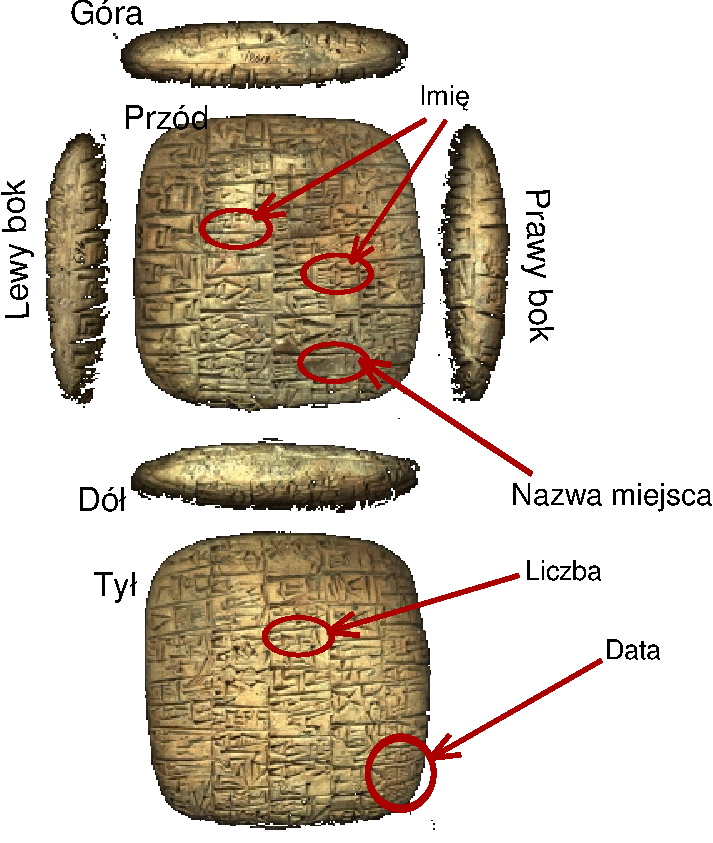
\includegraphics[width=150px]{../diagramy/tabliczka.pdf}
 % tabliczka.pdf: 342x405 pixel, 72dpi, 12.06x14.29 cm, bb=0 0 342 405
 \caption{\label{fig:tabliczka}Gliniana tabliczka -- struktura}
\end{wrapfigure}


% \begin{figure}[h]
%  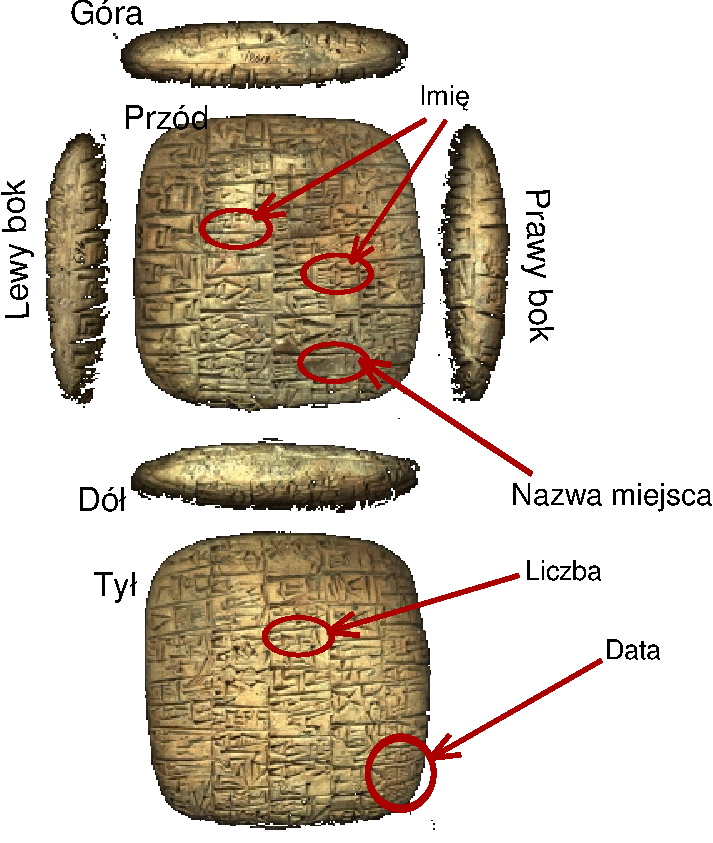
\includegraphics[width=150px]{../diagramy/tabliczka.pdf}
%  % tabliczka.pdf: 342x405 pixel, 72dpi, 12.06x14.29 cm, bb=0 0 342 405
%  \caption{Gliniana tabliczka - struktura}
% \end{figure}

\begin{figure}
 \centering
 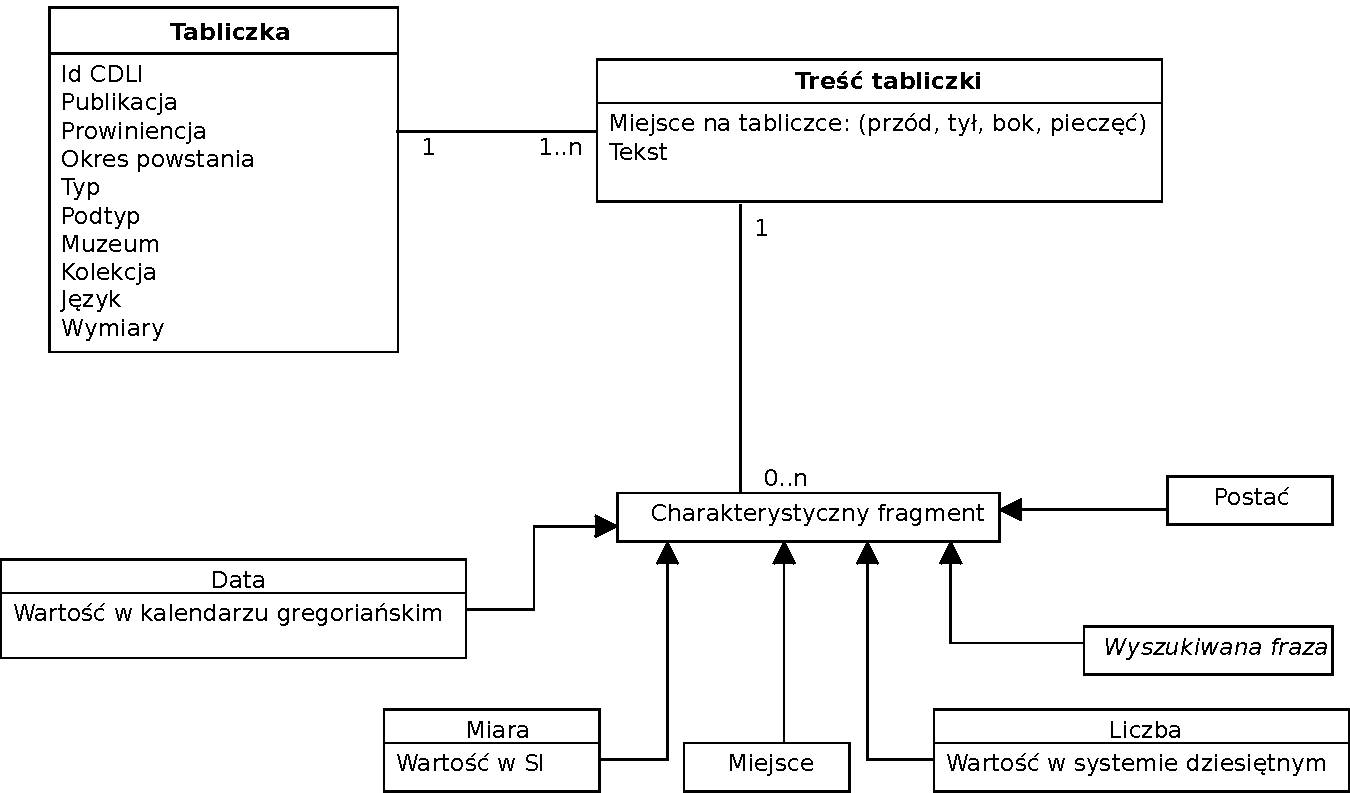
\includegraphics[width=400px]{../diagramy/Model-dziedziny.pdf}
 % Model-dziedziny.png: 650x345 pixel, 72dpi, 22.93x12.17 cm, bb=0 0 650 345
 \caption{Co powinna zawierać cyfrowa reprezantacja tabliczki}
\end{figure}
Podstawowym elementem rozpatrywanej przez nas dziedziny jest \emph{tabliczka sumeryjska}. 
Pojęcie to odnosi się zarówno do fizycznej \emph{tabliczki glinianej} jak i do jej cyfrowej reprezentacji, 
odpowiedniej do przechowywania na komputerze. 

Tabliczki gliniane mają różne kształty i rozmiary. 
Mogą być zapisane z wielu stron (z przodu, z tyłu, od góry, z boku, itp.), a także mogą zawierać pieczęcie, 
na których również znajduje się tekst. Przez kilka tysięcy lat istnienia ulegały też uszkodzeniom uniemożliwiającym 
obecnie ich pełne odczytanie.
Przykładowa gliniana tabliczka zaprezentowana jest na rysunku \ref{fig:tabliczka}.

% akapit o samym piśmie klinowym
Tekst na tabliczkach jest zapisany za pomocą \emph{klinów}. Pismo klinowe jest prawdopodobnie najstarszym pismem na świecie 
(konkurują z nim jedynie hieroglify egipskie)  \cite{kuckenburg}. Początkowo składało się z piktogramów z czasem coraz bardziej upraszczanych.
Służyło pomocą w rozliczeniach i umowach, zapisywano np. ilość i rodzaj obiecanych ludziom zwierząt.

Treść tabliczek to najczęściej dokumenty urzędowe dotyczące czynności administracyjnych i gospodarczych, 
produkcji i dystrybucji rozmaitych artykułów, uroczystości religijno--kulturowych, umów cywilnoprawnych itp. \cite{powalka}
Często można spotkać w niej między innymi imiona osób i bóstw, liczby, jednostki (np. mina -- jednostka wagi), % sprawdziłam
miejsca, daty. Niektóre z tych elementów można przetłumaczyć na współczesny język, na przykład jednostki można przeliczyć na SI, 
datę opisową na datę wg obecnego kalendarza gregoriańskiego. 

Dla ułatwienia pracy sumerolodzy tłumaczą zapis klinowy na tzw. \emph{odczyty}. 
Są one sposobem zapisania tekstu sumeryjskiego za pomocą współczesnych znaków -- liter alfabetu łacińskiego i cyfr arabskich, 
na podstawie prawdopodobnego brzmienia słów w języku sumeryjskim. 
W tłumaczeniu uwzględniony jest także kształt tabliczki i rozmieszczenie poszczególnych fragmentów tekstu 
(zgodnie z rysunkiem \ref{fig:tabliczka}). 
 
Odczyty zawarte w cyfrowym zapisie tabliczki są tylko jednym z wariantów tłumaczenia z klinów. 
Przede wszystkim dlatego, że jeden klin może zostać odczytany na wiele różnych sposobów. 
Ponadto odczytowi może odpowiadać nie tylko jeden klin, ale także ich sekwencja. 
Ponieważ w cyfrowej wersji nie ma klinów, trudno jest zweryfikować ewentualne pomyłki w tłumaczeniach.

W takiej właśnie formie tabliczki elektroniczne są przechowywane w pamięci komputerów. 
Niestety ten zapis może być mylący ze względu na niejednoznaczności występujące przy tłumaczeniu. 

% Pomocne mogłoby by narzędzie, które pozwala wyszukiwać również w alternatywnych tłumaczeniach.
Źródłem dodatkowych problemów są uszkodzenia tabliczek. 
W wielu przypadkach naukowcy mogą domyślić się jak wyglądał brakujący fragment. 
Zawsze natomiast informację o uszkodzeniu oraz domniemaną brakującą treść zapisują w tabliczce cyfrowej.
Ponieważ pewne konwencje opisywania tych informacji zostały przyjęte dosyć późno i nie przez wszystkich sumerologów, 
są one zapisywane na różne sposoby. Również tutaj możliwe są pomyłki i niejednoznaczności.

Tabliczka cyfrowa, oprócz treści, zawiera także informacje, które nie były zawarte na tabliczce glinianej. 
Są to metadane takie jak miejsce znalezienia tabliczki, okres, w którym powstała, czy nazwa kolekcji, do której obecnie należy. 
Te informacje są istotne przy przeszukiwaniu, gdyż często pozwalają na określenie o czym jest tabliczka bez dokładnej analizy 
jej treści. 
W praktyce, wśród sumerologów, atrybutem, który w znacznym stopniu pomaga zidentyfikować tabliczkę, jest informacja o jej publikacji.

Nie ma wątpliwości, że cyfrowa postać tabliczek sumeryjskich wraz z podstawowymi możliwościami wyszukiwania znacząco
ułatwia sumerologom ich badania. Brakuje im jednak możliwości znajdowania tabliczek na podstawie
bardziej skomplikowanych i rozbudowanych kryteriów.
Wychodząc naprzeciw tej potrzebie, chcemy stworzyć język, w którym będą oni mogli w łatwy sposób wyrażać, 
jakich tabliczek potrzebują, i który jednocześnie będzie można wykorzystać do przeszukiwania baz danych. 
Język ten powinien przede wszystkim umożliwiać wyszukiwanie na podstawie treści tabliczki (odczytów), 
alternatywnych tłumaczeń (wymaga to przetłumaczenia tabliczki z powrotem na kliny) oraz metadanych.
Dodatkową zaletą byłoby wyszukiwanie po specyficznych fragmentach (tagach), takich jak imiona, jednostki, daty.
W pierwszej wersji języka implementujemy tylko wyszukiwanie po odczytach i metadanych.
\chapter{Wcześniejsze rozwiązania}\label{r:losers}

% TODO: dlaczego nasze rozwiązanie jest najlepsze

W chwili obecnej nie istnieje język dostosowany do potrzeb sumerologów. Jedyne znane nam rozwiązania przedstawionego wyżej problemu opierają się o pomysł formularzy, które w łatwy sposób można wypełniać i łatwo na ich podstawie tworzyć zapytania. Wadą takich rozwiązań jest brak możliwości tworzenia skomplikowanych zapytań.
Poniżej przedstawimy dwie przykładowe strony internetowe oferujące wyszukiwanie za pomocą formularzy.
\section{The Cuneiform Digital Library Initiative \cite{cdli}}
\begin{figure}[h]
 \centering
 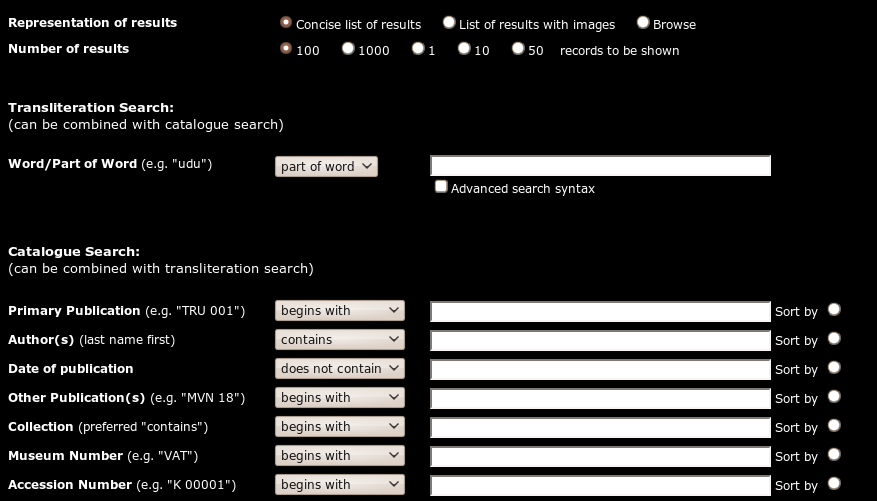
\includegraphics[width=300px]{../diagramy/cdli-search.png}
 % cdli-search.png: 877x501 pixel, 72dpi, 30.94x17.67 cm, bb=0 0 877 501
 \caption{Formularz wyszukiwania na stronie CDLI}
 \label{fig:cdli-search}
\end{figure}

CDLI to największa znana nam baza tekstów sumeryjskich, zawiera ok. 225 tys. tekstów. 
Umożliwia wyszukiwanie po wielu parametrach.
Dla każdej metadanej jest pole tekstowe z możliwymi opcjami wyszukiwania: ``begins with``, ``contains'', ''does not contain''. 
Dla treści jest pole tekstowe z opcjami ``word``, ``part of word``.
Jest również checkbox ''advanced search syntax'', jednak brakuje wyjaśnienia jak go używać.
Nie można tworzyć bardziej skomplikowanych warunków dla poszczególnych parametrów oraz zapytań złożonych.

\section{The Electronic Text Corpus of Sumerian Literature \cite{etcsl}} 
\begin{figure}[h]
 \centering
 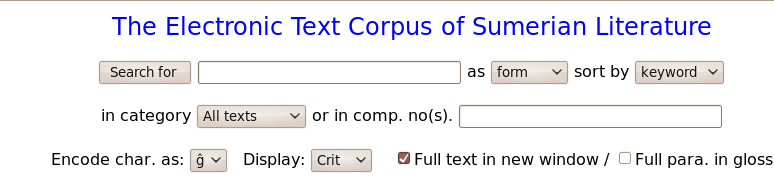
\includegraphics[width=300px]{../diagramy/etcsl-search.png}
 % etcsl-search.png: 774x182 pixel, 72dpi, 27.31x6.42 cm, bb=0 0 774 182
 \caption{Formularz wyszukiwania na stronie ETCSL}
 \label{fig:etcsl-search}
\end{figure}

ETCSL jest znacznie mniejszą bazą, zawierającą głównie teksty literackie. 
Ma ograniczone możliwości wyszukiwania po metadanych (tylko po kategorii tekstu), jednak udostępnia tworzenie bardziej 
skomplikowanych zapytań dotyczące treści tabliczki. 
Pozwala określić typ wyszukiwanego słowo (form, lemma, label, pos, emesal, sign),
 a także jego znaczenie w tekście (np. czy jest imieniem bóstwa) oraz część mowy, do której należy. 
Można również wyszukiwać po fragmencie słowa.


\part{Definicja języka TQL}
\chapter{Definicja języka TQL}
\section{Tablets Query Language}
Tablets Query Language (TQL) jest naszą propozycją rozwiązania problemu wyszukiwania tabliczek sumeryjskich.
Jest to zewnętrzny język dziedzinowy stworzony do tego, aby służyć sumerologom jako język zapytań.
Formalna definicja składni TQL znajduje się w rozdziale \ref{chap:skladnia}.
Jest ona zaprojektowana od podstaw, dzięki czemu jest bardzo prosta i intuicyjna, co będzie widać na przykładach 
opisujących semantykę w rozdziale \ref{chap:semantyka}. 
Wiele języków dziedzinowych, w przeciwieństwie do TQL, bazuje na istniejących już językach. Są to tzw. wewnętrzne języki dziedzinowe. Jednak w przypadku naszego problemu było to niewskazane rozwiązanie, gdyż składnia przejęta z istniejącego języka zapytań bardziej ogólnego zastosowania byłaby nieintuicyjna, a tworzone zapytania długie i skomplikowane.
Udało nam się połączyć prostą składnię TQL z dużą siłą wyrazu.
 Język daje możliwość formułowania złożonych 
wyrażeń do wyszukiwania na podstawie pojedynczej
metadanej lub treści tabliczki oraz możliwość łączenia wielu zapytań w jedno.

Dodatkowo, jednym z głównych założeń przyjętych przy tworzeniu języka TQL jest niezależność od rzeczywistej
reprezentacji danych. Przy konstruowaniu go nie brałyśmy pod uwagę sposobu fizycznej reprezentacji tabliczek,
czyli rodzaju bazy danych oraz schematu danych. Skupiłyśmy się jedynie na dziedzinie problemu, czyli na tym,
co zawiera tabliczka oraz na podstawie jakich informacji chcemy wyszukiwać. Zakładamy, że niezależnie od
reprezentacji danych takie wyszukiwanie będzie możliwe, chociaż oczywiście skonstruowanie odpowiedniego
zapytania może być skomplikowane. Przetłumaczenie zapytania TQL na zapytanie w języku odpowiednim do
reprezentacji danych, np. SQL, XQuery, jest zadaniem programu tłumaczącego. Dzięki temu praca polegająca
na przetłumaczeniu zapytania z "języka dziedziny" na "język komputerów" jest wykonana tylko raz dla każdego
sposobu reprezentacji danych, i to przez programistów, a nie sumerologów.

Język TQL umożliwia wyszukiwanie na podstawie kryteriów dotyczących następujących danych:
\begin{longtable}{|p{3in}|p{2.5in}|}
\hline
{\bf Opis} & {\bf Nazwa pola w TQL}\\
\hline
\endhead
numer tabliczki w bazie CDLI & cdli\_id
\\
\hline
miejsce pochodzenia (proweniencja) & provenience
\\
\hline
okres powstania & period
\\
\hline
typ i podtyp & genre
\\
\hline
rok powstania & year
\\
\hline
publikacja & publication
\\
\hline
treść (odczyty)& text
\\
\hline
%treść (kliny) & cunetext
%\\
%\hline
kolekcja & collection
\\
\hline
muzeum & museum
\\
\hline
\end{longtable}
Język można łatwo rozszerzać, aby umożliwić tworzenie kryteriów wyszukiwania w oparciu o inne dane
(np. kliny, zawartość pieczęci).

W kolejnych dwóch rozdziałach przedstawimy gramatykę i semantykę zaprojektowanego przez nas języka TQL.



\section{\label{chap:skladnia}Gramatyka}

W tym rozdziale przedstawimy gramatykę zaprojektowanego przez nas języka.
W pierwszej części pokażemy strukturę leksykalną TQL, czyli elementy, z których buduje się zapytania.
W drugiej części zaprezentujemy reguły tworzenia zapytań, zapisane w formie reguł gramatyki w notacji BNF.

\subsection{Struktura leksykalna}

\subsubsection{Literały}

% \paragraph{String}
Literał \terminal{String}\ jest ciągiem dowolnych znaków w cudzysłowie (\texttt{"}). Nie może zawierać jedynie znaków
``\texttt{"}`` niepoprzedzonych ''\verb6\6``.

% \paragraph{SłowoOdLitery}
Literał \terminal{SłowoOdLitery} to ciąg liter, cyfr oraz znaków {''\texttt{-}``, ''\texttt{'}``, ''\texttt{\_}``},
zaczynający się od litery, z wyjątkiem słów kluczowych.

% \paragraph{SłowoOdLiczby}
Literał \terminal{SłowoOdLiczby} to ciąg liter, cyfr oraz znaków {''\texttt{-}``, ''\texttt{'}``, ''\texttt{\_}``},
zaczynający się od cyfry.


\subsubsection{Słowa kluczowe}

\begin{tabular}{lll}
{\reserved{as}} &{\reserved{define}} &{\reserved{in}} \\
{\reserved{search}} & & \\
\end{tabular}\\

\subsubsection{Znaki specjalne}

\begin{tabular}{lll}
{\symb{(}} &{\symb{)}} &{\symb{{$+$}}} \\
{\symb{/}} &{\symb{{$-$}{$-$}}} &{\symb{*}} \\
{\symb{:}} & &{\symb{$\backslash$n}} (koniec linii)\\
\end{tabular}\\

\subsection{\label{sec:skladnia}Struktura składniowa języka}

Poniżej przedstawimy reguły gramatyki TQL w notacji BNF.
Nieterminale są zapisane pomiędzy ''$\langle$`` a ''$\rangle$``.
Symbole ''{\arrow}`` (produkcja), ''{\delimit}`` (lub)
i ''{\emptyP}`` (pusta reguła) należą do notacji BNF.
Wszystkie pozostałe symbole to terminale.\\

\begin{tabular}{lll}
{\nonterminal{Zapytanie Złożone}} & {\arrow} &{\nonterminal{Lista Zapytań}} \\
\end{tabular}\\

\begin{tabular}{lll}
{\nonterminal{Lista Zapytań}} & {\arrow} &{\nonterminal{Zapytanie}} \\
 & {\delimit} &{\nonterminal{Zapytanie}} {\nonterminal{Lista Zapytań}} \\
\end{tabular}\\

\begin{tabular}{lll}
{\nonterminal{Zapytanie}} & {\arrow} &{\nonterminal{Lista Linii Zapytania}} {\nonterminal{Lista Pustych Linii}} \\
 & {\delimit} &{\terminal{define}} {\terminal{$\backslash$n}} {\nonterminal{Zapytanie}} {\terminal{as}} {\nonterminal{Nazwa}} {\nonterminal{Lista Pustych Linii}} \\
 & {\delimit} &{\terminal{search}} {\terminal{$\backslash$n}} {\nonterminal{Zapytanie}} {\terminal{in}} {\nonterminal{Nazwa}} {\nonterminal{Lista Pustych Linii}} \\
  & {\delimit} &{\terminal{search}} {\nonterminal{Nazwa}} {\nonterminal{Lista Pustych Linii}} \\
 & {\delimit} &{\nonterminal{Lista Pustych Linii}} \\
\end{tabular}\\

\begin{tabular}{lll}
{\nonterminal{Lista Linii Zapytania}} & {\arrow} &{\nonterminal{Linia Zapytania}} {\terminal{$\backslash$n}} \\
 & {\delimit} &{\nonterminal{Linia Zapytania}} {\terminal{$\backslash$n}} {\nonterminal{Lista Linii Zapytania}} \\
\end{tabular}\\

\begin{tabular}{lll}
{\nonterminal{Linia Zapytania}} & {\arrow} &{\nonterminal{Nazwa pola}} {\terminal{:}} {\nonterminal{Wyrażenie}} \\
\end{tabular}\\

\begin{tabular}{lll}
{\nonterminal{Wyrażenie}} & {\arrow} &{\nonterminal{Wyrażenie}} {\terminal{{$+$}}} {\nonterminal{Wyrażenie1}} \\
 & {\delimit} &{\nonterminal{Wyrażenie}} {\terminal{/}} {\nonterminal{Wyrażenie1}} \\
 & {\delimit} &{\nonterminal{Wyrażenie1}} \\
\end{tabular}\\

\begin{tabular}{lll}
{\nonterminal{Wyrażenie1}} & {\arrow} &{\terminal{{$-$}{$-$}}} {\nonterminal{Wyrażenie1}} \\
 & {\delimit} &{\nonterminal{Wyrażenie2}} \\
\end{tabular}\\

\begin{tabular}{lll}
{\nonterminal{Wyrażenie2}} & {\arrow} &{\nonterminal{Wyrażenie3}} {\terminal{*}} {\nonterminal{Wyrażenie3}} \\
 & {\delimit} &{\nonterminal{Tekst}} \\
 & {\delimit} &{\terminal{(}} {\nonterminal{Wyrażenie}} {\terminal{)}} \\
\end{tabular}\\

\begin{tabular}{lll}
{\nonterminal{Wyrażenie3}} & {\arrow} &{\nonterminal{Wyrażenie2}}\\
 & {\delimit} &{\emptyP} \\
\end{tabular}\\

\begin{tabular}{lll}
{\nonterminal{Lista Pustych Linii}} & {\arrow} &{\emptyP} \\
 & {\delimit} &{\nonterminal{Pusta Linia}} {\nonterminal{Lista Pustych Linii}} \\
\end{tabular}\\

\begin{tabular}{lll}
{\nonterminal{Pusta Linia}} & {\arrow} &{\terminal{$\backslash$n}} \\
\end{tabular}\\

\begin{tabular}{lll}
{\nonterminal{Tekst}} & {\arrow} &{\terminal{String}} \\
 & {\delimit} &{\nonterminal{Słowo}} \\
\end{tabular}\\

\begin{tabular}{lll}
{\nonterminal{Słowo}} & {\arrow} &{\terminal{SłowoOdLitery}} \\
 & {\delimit} &{\terminal{SłowoOdLiczby}} \\
\end{tabular}\\

\begin{tabular}{lll}
{\nonterminal{Nazwa pola}} & {\arrow} &{\terminal{SłowoOdLitery}} \\
\end{tabular}\\

\begin{tabular}{lll}
{\nonterminal{Nazwa}} & {\arrow} &{\terminal{String}} \\
\end{tabular}\\

Powyższa gramatyka jest gramatyką bezkontekstową.

\section{\label{chap:semantyka}Semantyka}

Poniżej przedstawiamy semantykę wybranych przykładów.
\subsection{Zapytanie proste}
\begin{verbatim}
provenience: Gar*
period: "Ur III"
genre: Administrative
text: udu + (masz2/ugula) --szabra
\end{verbatim}
Wynikiem zapytania będą wszystkie tabliczki, które:
\begin{itemize}
\item pochodzą z miejscowości o nazwie zaczynającej się na ``Gar''
\item pochodzą z okresu Ur III
\item są dokumentami administracyjnymi
\item zawierają słowo ``udu'' oraz conajmniej jedno ze słów ``masz2'' lub ``ugula''
\item nie zawierają słowa ``szabra''.
\end{itemize}


\subsection{Zapytanie złożone}
\begin{verbatim}
provenience: Ur
period: "Ur III"/"Ur IV"
text: udu --szabra

text: masz2/ugula
publication: *tan
provenience: Ur
\end{verbatim}
Wynikiem zapytania będą wszystkie tabliczki, które:
\begin{itemize}
 \item pochodzą z miejscowości Ur
 \item pochodzą z okresu Ur III lub Ur IV
 \item zawierają słowo ``udu''
 \item nie zawierają słowa ``szabra``
\end{itemize}
oraz wszystkie tabliczki, które:
\begin{itemize}
 \item zawierają słowo ''masz2`` lub ''ugula``
 \item zostały opublikowane w pracy, której nazwa kończy się na ''tan``
 \item pochodzą z miejscowości Ur.
\end{itemize}


\subsection{\label{sec:zdefiniowane} Zapytanie zdefiniowane}
\begin{verbatim}
 define
  provenience: Gar*a
  period: Ur III
  text: "udu ban"/mash2
as "zwierzęta w Gar*a"
\end{verbatim}
Wynikiem zapytania (po jego wywołaniu) będą wszystkie tabliczki, które:
\begin{itemize}
\item pochodzą z miejscowości, których nazwy zaczynają się na ''Gar`` i kończą na ''a''
\item pochodzą z okresu Ur III
\item zawierają conajmniej jedną z fraz ''udu ban`` lub ''mash2``.
\end{itemize}

\subsection{Wywołanie zapytania zdefiniowanego}
\subsubsection{Zwykłe}
\begin{verbatim}
search "zwierzęta w Gar*a"
\end{verbatim}
Wynikiem zapytania będą dokładnie te tabliczki, które spełniają wszystkie warunki zapytania ''zwierzęta w Gar*a``.\\
Takie zapytanie jest równoważne następującemu zapytaniu prostemu:
\begin{verbatim}
  provenience: Gar*a
  period: Ur III
  text: "udu ban"/mash2
\end{verbatim}
Zakładając, że \textit{''zwierzęta w Gar*a``} są jak w sekcji \ref{sec:zdefiniowane}.
\subsubsection{Z dodatkowym warunkiem wyszukiwania}
\begin{verbatim}
search
  text: adad-tilati
in "zwierzęta w Gar*a"
\end{verbatim}
Wynikiem zapytania będą wszystkie tabliczki, które:
\begin{itemize}
 \item spełniają wszystkie warunki zapytania ''zwierzęta w Gar*a``
\item zawierają słowo ''adad--tilati``.
\end{itemize}
% Łatwo zauważyć, że jest to część wspólna zbiorów wyników dwóch zapytań prostych. 
% Jedno z nich to wnętrze zapytania zdefiniowanego, a drugie to dodatkowe warunki wyszukiwania.
Takie zapytanie jest równoważne następującemu zapytaniu prostemu:
\begin{verbatim}
  provenience: Gar*a
  period: Ur III
  text: ("udu ban"/mash2)+adad-tilati
\end{verbatim}
Zakładając, że \textit{''zwierzęta w Gar*a``} są jak w sekcji \ref{sec:zdefiniowane}.



\part{Implementacja}
\begin{figure}[h]
 \centering
 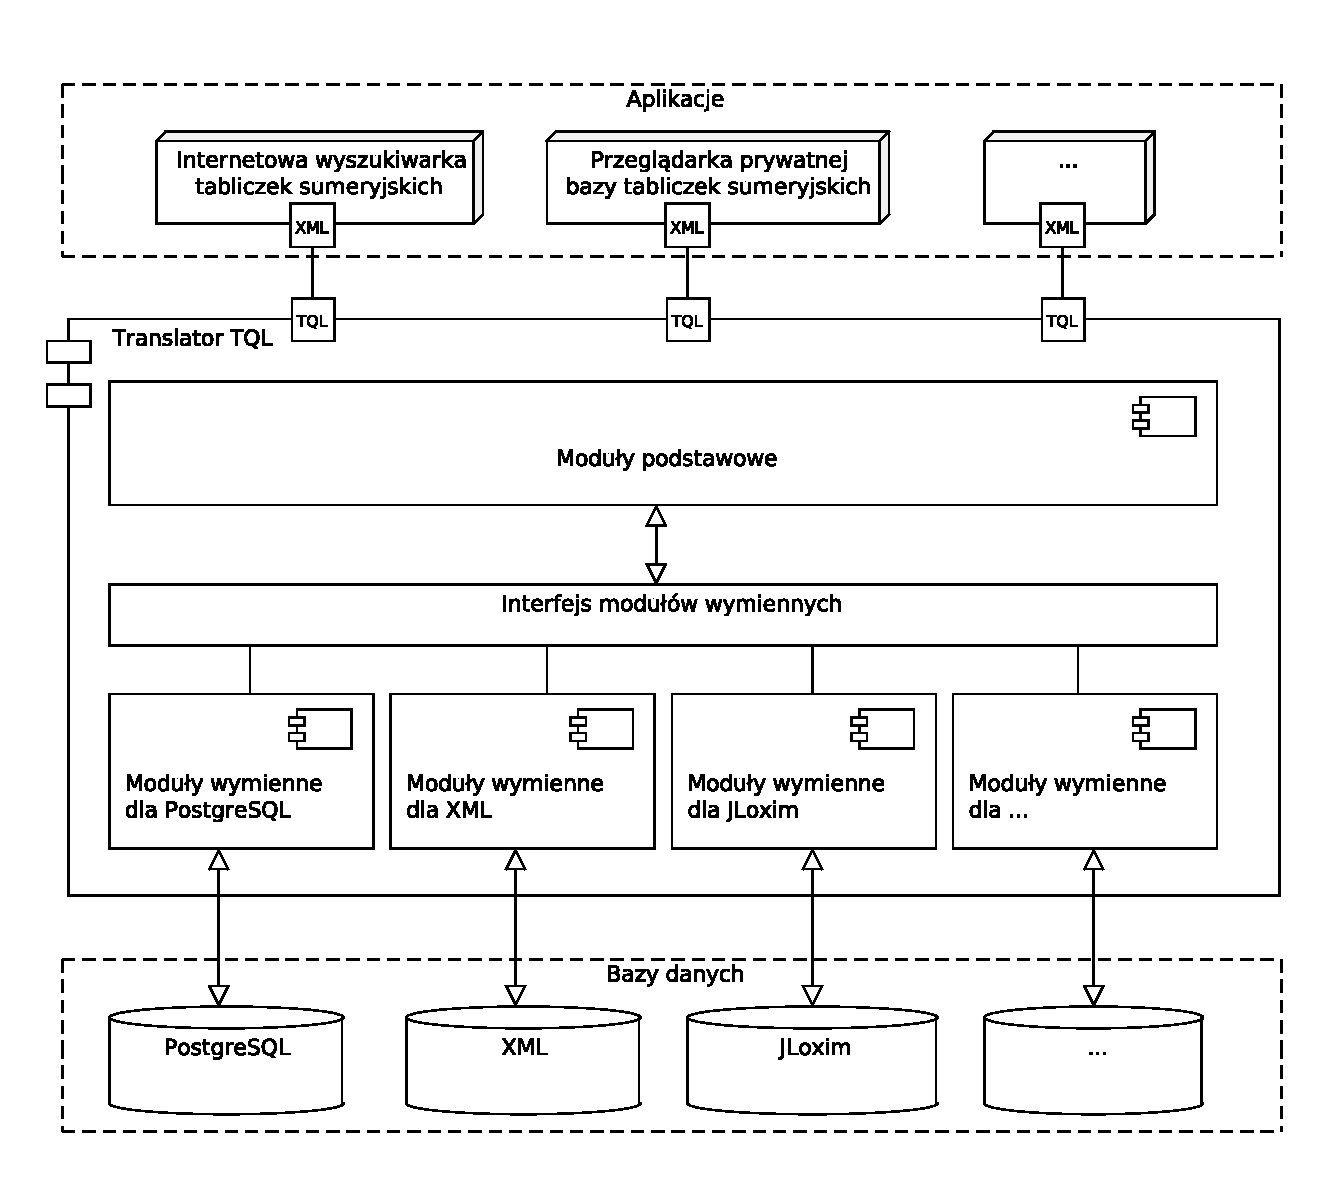
\includegraphics[width=450px,bb=0 0 608 517]{../diagramy/struktura2.pdf}
 % struktura.pdf: 608x517 pixel, 72dpi, 21.45x18.24 cm, bb=0 0 608 517
 \caption{Struktura systemu korzystającego z translatora}
\end{figure}

\begin{figure}
 \centering
 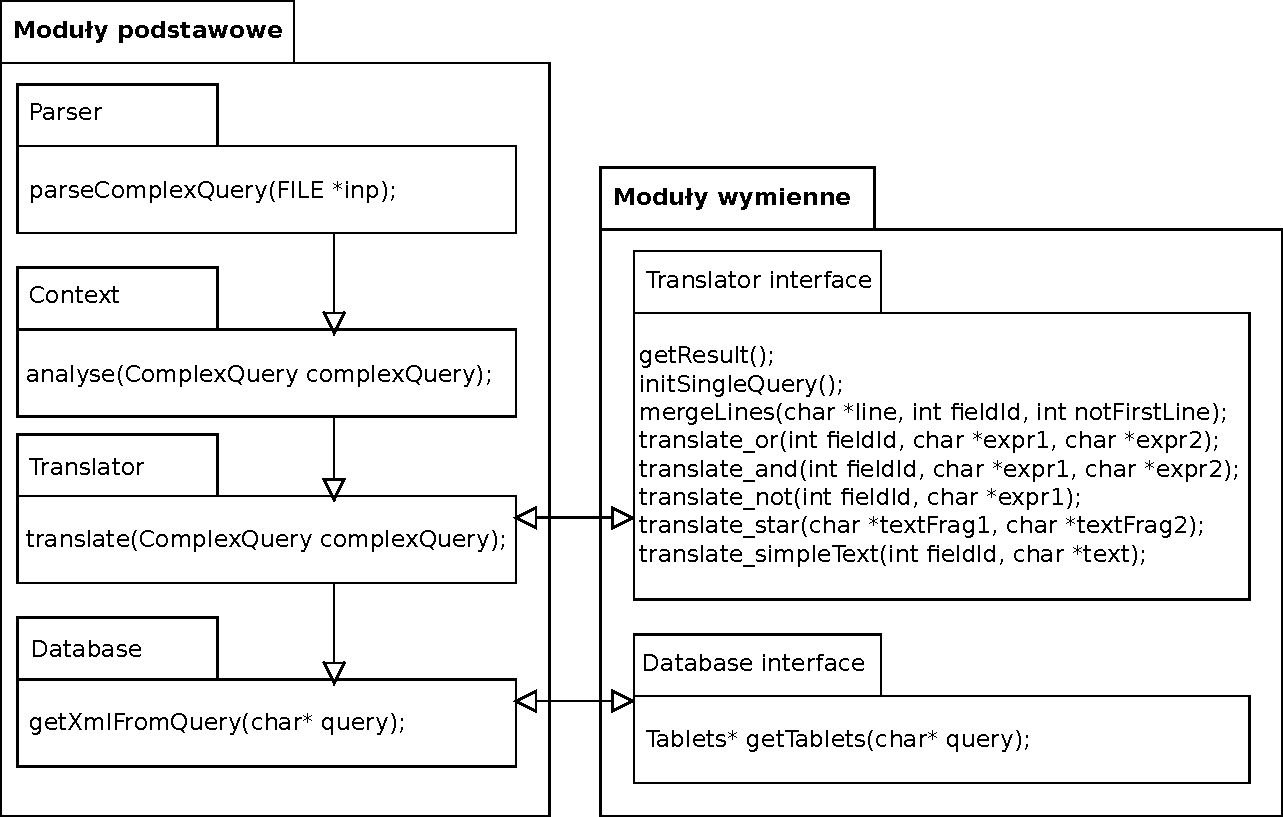
\includegraphics[width=500px]{../diagramy/pakiety.pdf}
 % pakiety.pdf: 585x300 pixel, 72dpi, 20.64x10.58 cm, bb=0 0 585 300
 \caption{Podział programu na moduły}
\end{figure}
Jednym z głównych założeń języka TQL, szczególnie ważnym z punktu widzenia implementacji, jest niezależność od struktury danych.
W związku z tym istotną cechą translatora jest możliwość dostosowania do współpracy z różnymi bazami danych.
%Jednym z głównych wymagań postawionych przed translatorem, żeby można było podłączyć różne bazy danych.
 Wynikiem tego jest podział translatora na 2 rodzaje modułów:
\begin{enumerate}
 \item \textbf{Podstawowe} -- niezależne od struktury danych i zajmujące się głównie parsowaniem i analizą składniową zapytania.
 \item \textbf{Wymienne} -- zależne od struktury danych, tłumaczące zapytanie TQL na język odpowiedni dla używanej bazy danych
i wywołujące je.
\end{enumerate}
 W niniejszej pracy przedstawiamy dwie prototypowe implementacje, zawierające własne zestawy modułów wymiennych:
  \begin{itemize}
   \item dla bazy PostgreSQL
   \item dla bazy XML
  \end{itemize}
  Wybór modułów wymiennych odbywa się na poziomie kompilacji. Stworzony przez nas makefile domyślnie buduje obie implementacje translatora TQL.
%Bez względu na wybór modułu wymiennego interfejs całego translatora jest taki sam we wszystkich instancjach.


\chapter{Moduły podstawowe}

\section{Parser}
Parser został utworzony za pomocą narzędzia BNFC \cite{bnfc}. Następnie zostały w nim wprowadzone modyfikacje:
\begin{itemize}
\item poprawienie nazw stałych oznaczających symbole na bardziej intuicyjne,
\item dodanie tablicy symboli,
\item usunięcie niepotrzebnych funkcji z interfejsu,
\item uporządkowanie kodu.
\end{itemize}
Moduł ten parsuje zapytanie w języku TQL, tworząc drzewo struktury składniowej, które jest zdefiniowane w pliku pomocniczym Absyn.h.
Na parser składają się następujące pliki:
\begin{itemize}
 \item Parser.cpp
 \item Parser.h
 \item TQL.y % tłumaczony na Parser.c
 \item TQL.l % tłumaczony na Lexer.c
\end{itemize}

\section{Analizator kontekstowy}
Moduł analizuje drzewo struktury składniowej w następujący sposób:
\begin{itemize}
 \item sprawdza, czy podano prawidłowe nazwy pól,  %to co jest po lewej w linii zapytania jest nazwą pola.
\item upraszcza drzewo - z wywołania zapytania (wywołanie \textit{search in}) tworzy zapytanie proste.
\end{itemize}
Składa się z następujących plików:
\begin{itemize}
 \item Context.cpp
 \item Context.h
\end{itemize}

\section{Translator}
Zadaniem translatora jest przetłumaczenie drzewa składni abstrakcyjnej na zapytanie w docelowym języku. 
Składa się z następujących plików:
\begin {itemize}
 \item Translator.cpp
 \item Translator.h
 \item Translator\_interface.h (interfejs modułu translatora zależnego od bazy danych)
 %\item Translator\_config.c (implementacja interfejsu z Translator\_config.h, zależny od wyboru bazy danych itp)
\end {itemize}

Tłumaczenie poszczególnych elementów drzewa zależy od implementacji interfejsu zawartego w pliku Translator\_interface.h. 
Funkcja translate() przechodzi całą strukturę drzewa, wywołując w razie potrzeby odpowiednie funkcje z Translator\_interface.
Następnie pobiera przetłumaczone zapytanie za pomocą funkcji getResult(), aby przekazać je do modułu bazy.

\section{Baza}
Moduł bazy jest odpowiedzialny za wywołanie przetłumaczonego zapytania i przekazanie wyniku w określonej formie - jako XML.
Składa się z następujących plików:
\begin {itemize}
 \item Database.cpp
 \item Database.h
 \item Database\_interface.h (interfejs modułu bazy zależnego od bazy danych)
% \item Database\_config.c (implementacja interfejsu z Database\_conf.h, zależny od wyboru bazy danych itp)
\end {itemize}

Wywołuje funkcję getTablets() z Database\_interface.h, jako parametr podając przetłumaczoną treść zapytania. 
Funkcja ta zwraca strukturę danych Tablets, wypełnioną informacjami o wyszukanych tabliczkach.
Następnie na podstawie otrzymanej struktury moduł tworzy dokument XML.
\newline
Definicja struktury Tablets:
\begin{verbatim}
typedef struct{    
    char* id;
    char* id_cdli;
    char* publication;
    char* measurements;
    char* year;
    char* provenience;
    char* period;
    char* genre;
    char* subgenre;
    char* collection;
    char* text;
    Tags* tags; // specjalnie oznaczone miejsca w tekscie
                // (w pierwszej wersji frazy wyszukiwania)
} Tablet;

typedef struct{
    int size;
    Tablet* tabs;
} Tablets;
\end{verbatim}

%//miejsca gdzie w tekście są wyniki wyszukiwania

%Wszystkie niezbędne informacje powinny się znajdować w bazie danych.

\section{Pliki pomocnicze}
% TODO: wytłumaczyć co to jest BNFC??
Definicje struktur danych i funkcji służących do budowy drzewa struktury składniowej (wygenerowane za pomocą BNFC \cite{bnfc}, następnie uproszczone):
\begin{itemize}
 \item Absyn.cpp
 \item Absyn.h
\end{itemize}
Tablica symboli:
\begin{itemize}
 \item Symbols.cpp
\item Symbols.h
\end{itemize}
Obsługa błędów:
\begin{itemize}
 \item Err.cpp
\item Err.h
\end{itemize}
Moduł do dzielenia tekstu względem separatora, pobrany z internetu \cite{cexplode}:
\begin{itemize}
 \item Cexplode.cpp
 \item Cexplode.h
\end{itemize}


\chapter{Moduły wymienne}
Pliki zależne od wyboru konkretnej bazy danych to:
\begin{itemize}
 \item Translator\_$<$nazwa$>$.cpp - dla modułu translatora
\item Database\_$<$nazwa$>$.cpp - dla modułu bazy
\end{itemize}
Ich interfejsy są wspólne dla wszystkich baz danych.

\section{Baza PostgreSQL}
\subsection{Diagram encji}
\begin{figure}[h]
 \centering
 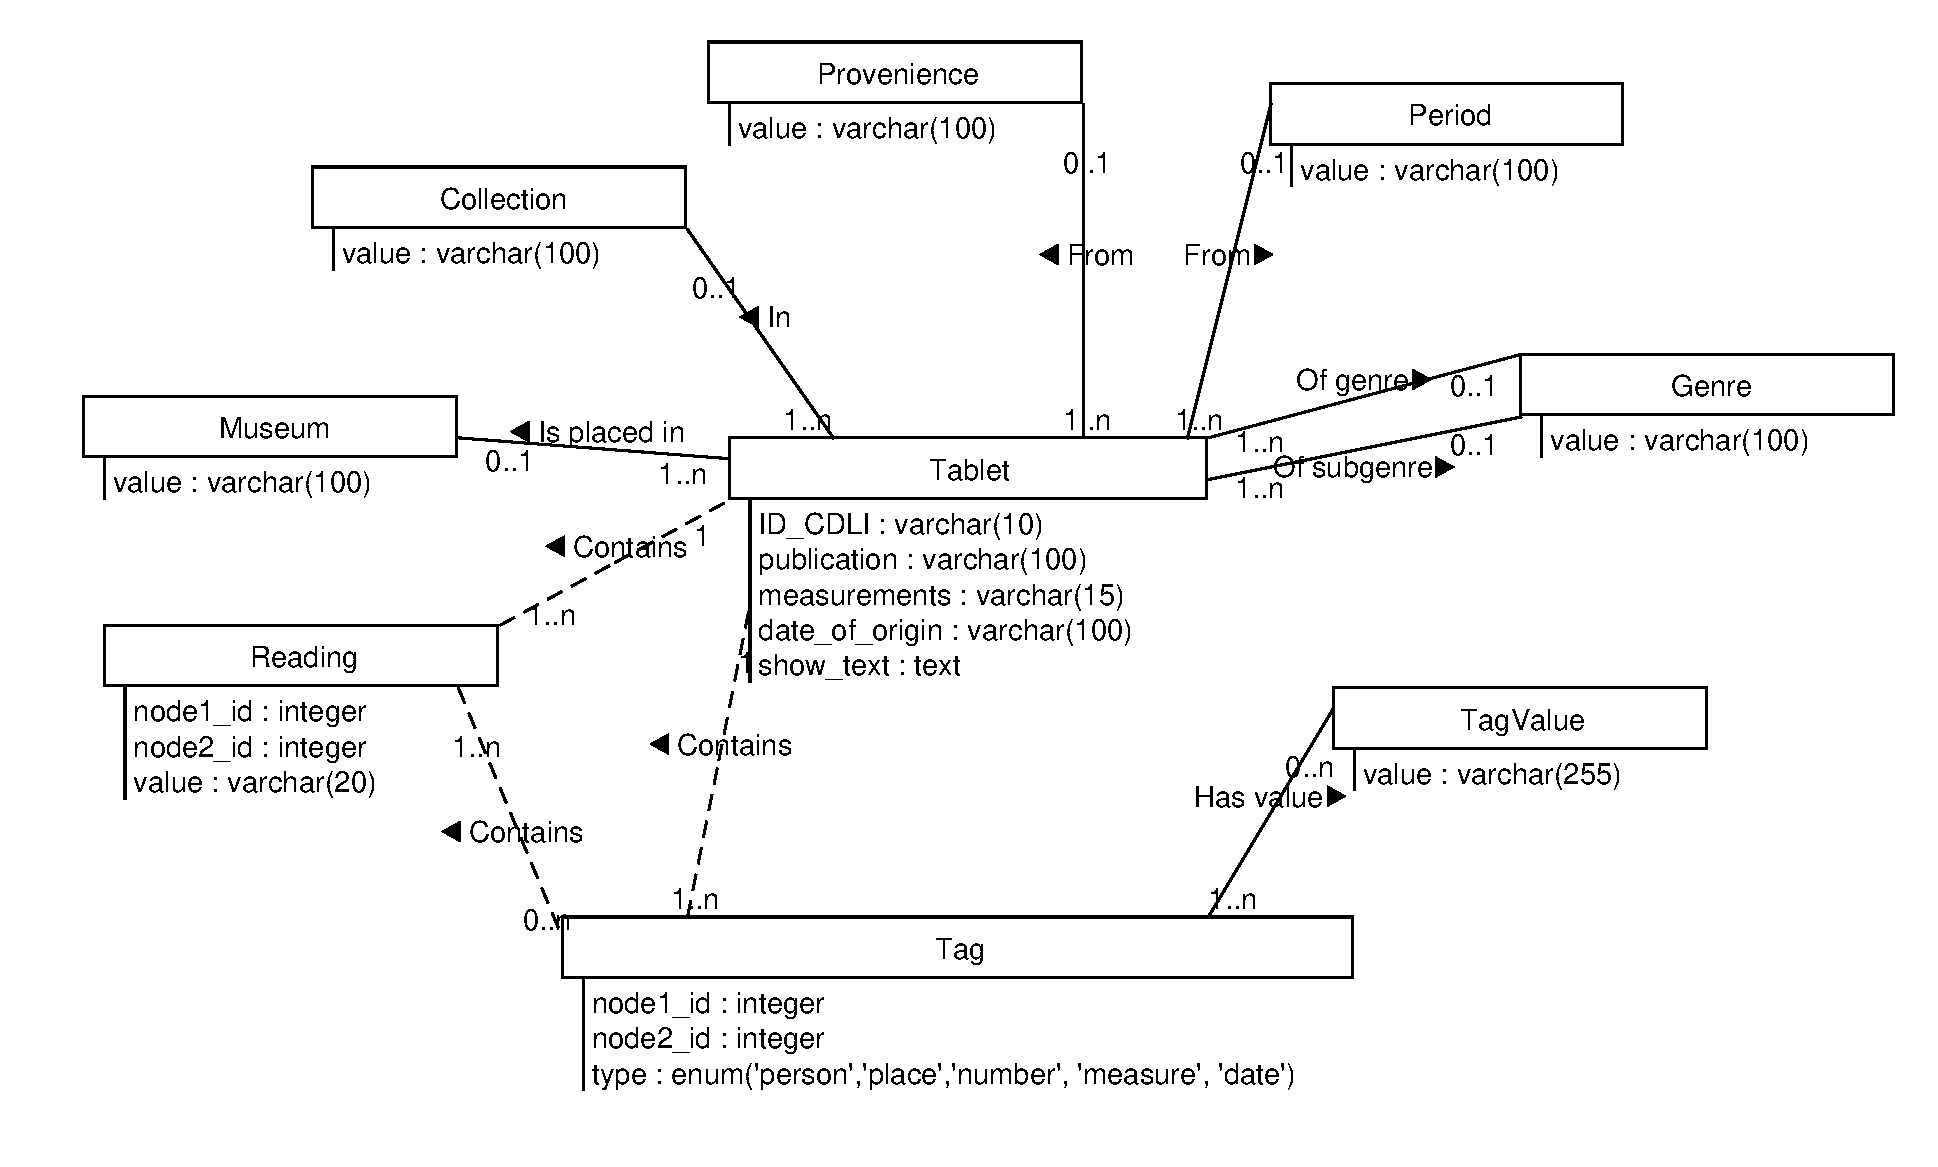
\includegraphics[width=500px,bb=0 0 930 560]{../diagramy/diagram-encji-maly.pdf}
 % diagram-encji-maly.pdf: 930x560 pixel, 72dpi, 32.81x19.76 cm, bb=0 0 930 560
 \caption{Diagram encji}
\end{figure}
Jednym z problemów przy projektowaniu bazy danych był wybór takiej reprezentacji treści tabliczki, 
żeby efektywnie wyszukiwać zarówno treść konkretnej tabliczki jak i tabliczki, których treść spełnia podane kryteria
 (wg odczytów lub zapisu klinowego).

W przypadku pierwszego problemu jako rozwiązanie narzuca się przechowywanie treści
jako otwarty tekst.
Natomiast najlepszym rozwiązaniem drugiego jest reprezentacja treści tabliczki
w formie grafu, którego krawędziami są odczyty i kliny (zgodnie z pomysłem dr Wojciecha Jaworskiego\cite[s.13-24]{jaworski}).
Zdecydowałyśmy się na połączenie obu sposobów. Odczyty oraz kliny przechowujemy w tabelach Reading i Cuneiform, 
natomiast otwarty tekst w kolumnie show\_text tabeli Tablet. 
% TODO: chyba trochę lepiej
Dzięki temu rozwiązaniu, szukając tabliczki zawierającej podane odczyty (lub kliny) korzystamy z reprezentacji
grafowej w tabelce Reading (lub Cuneiform).
Natomiast zawsze korzystamy z reprezentacji otwartym tekstem w tabelce Tablet w celu wyświetlenia treści tabliczki.
% Aby zapewnić możliwość odwzorowania treści tabliczki między reprezentacjami, węzły są liczbami postaci:
Kiedy więc wyszukujemy w tabelce Reading (lub Cuneiform) musimy być wstanie powiązać znalezione odczyty (kliny) 
z całą treścią tabliczki w tabeli Tablet. Osiągamy to zapisując węzły w grafie w postaci:
\begin{verbatim}
 <numer węzła w tabliczce> * 1 000 000 + <id tabliczki>
\end{verbatim}
gdzie numer węzła w tabliczce to numer kolejnego słowa (słowa są oddzielone spacjami i końcem linii) pomnożone przez 10 
(żeby umożliwić wstawienie kilku węzłów w jednym słowie np. pozwolić na przetłumaczenie jednego słowa na sekwencję trzech klinów). 


Przerywane linie na diagramie encji oznaczają opisany powyżej związek pomiędzy id węzła (node1\_id i node2\_id) 
a id tabliczki (Tablet.id).

% relacja
% Stąd wzięły się przerywane linie na diagramie encji - nie ma bezpośredniego klucza obcego w tabeli Reading (czy Tag) do Tablet, 
% jednak związek istnieje. Taki sposób przechowywania informacji o treści tabliczki umożliwia sprawniejsze wyszukiwanie nie tylko
% po odczytach (pozwala pomijać linie z uszkodzeniami) ale także w przyszłości ułatwia zaimplementowanie wyszukiwania po klinach,
% po tagach itp.
% Poza sprawnym
%  wyszukiwaniem ułatwia to rozszerzenie programu o możliwość wyszukiwania po klinach - po dodaniu tabeli Cuneiform.

 

\subsection{Translator\_postgres}
Tłumaczy otrzymane fragmenty drzewa struktury zapytania na język SQL. Przetłumaczone fragmenty zbiera do buforów 
(\textit{select}, \textit{from}, \textit{where}), które następnie odpowiednio łączy.
Każde proste zapytanie TQL jest tłumaczone na pojedyncze zapytanie SQL. Tłumaczenie kilku prostych zapytań
łączone jest za pomocą UNION.

\subsubsection{Stałe fragmenty zapytania}
Tłumaczenie prostego zapytania zaczyna się od inicjalizacji buforów przechowujących poszczególne części wynikowego SQL-a.\\
\textit{select} jest inicjowany na 
\begin{verbatim}
SELECT t.id, t.id_cdli, t.publication, t.measurements, t.origin_date, 
       p.value as provenience, pd.value as period,
       g1.value as genre, g2.value as subgenre, 
       c.value as collection, t.text
\end{verbatim}
\textit{from} jest inicjowany
\begin{verbatim}
FROM tablet t
  LEFT JOIN provenience p ON p.id = t.provenience_id
  LEFT JOIN collection c ON c.id = t.collection_id
  LEFT JOIN genre g1 ON g1.id = t.genre_id
  LEFT JOIN genre g2 ON g2.id = t.subgenre_id
  LEFT JOIN period pd ON pd.id = t.period_id
\end{verbatim}
\textit{where} początkowo zawiera pusty ciąg znaków.



\subsubsection{Tłumaczenie zapytań o atrybuty tabliczki}
Poniższe tłumaczenia są dodawane do bufora \textit{where} i łączone za pomocą AND.
\begin{longtable}{|p{3in}|p{3in}|}
\hline
{\bf Konstrukcja} & {\bf Tłumaczenie na SQL}\\
\hline
\endhead
provenience: wartosc & \begin{verbatim}p.value LIKE 'wartosc'\end{verbatim}
\\
\hline
publication: wartosc & 
\begin{verbatim}
t.publication LIKE 'wartosc'
\end{verbatim}
\\
\hline
period: wartosc & 
\begin{verbatim}
pd.value LIKE 'wartosc'
\end{verbatim}
\\
\hline
year: wartosc & 
\begin{verbatim}
t.origin_date LIKE 'wartosc'
\end{verbatim}
\\
\hline
genre: wartosc & 
\begin{verbatim}
   g1.value LIKE 'wartosc' 
OR g2.value LIKE 'wartosc'
\end{verbatim}
\\
\hline
cdli\_id: wartosc & 
\begin{verbatim}
t.cdli_id LIKE 'wartosc'
\end{verbatim}
\\
\hline
museum: wartosc & 
\begin{verbatim}
t.museum LIKE 'wartosc'
\end{verbatim}
\\
\hline
collection: wartosc & 
\begin{verbatim}
c.value LIKE 'wartosc'
\end{verbatim}
\\
\hline
\end{longtable}

\textbf{Tłumaczenie operatorów:}
\begin{longtable}{|p{1in}|p{1in}|}
\hline
{\bf Operator} & {\bf Tłumaczenie}\\
\hline
\endhead
/ & OR\\ 
\hline
-- & NOT\\ 
\hline
+ & AND\\ 
\hline
* & \%  \\ 
\hline
\end{longtable}


\subsubsection{Tłumaczenie zapytań o treść tabliczki}
Przy tłumaczeniu zapytań o treść tabliczki
korzystamy z przedstawienia treści tabliczki w formie grafu.

Pojawienie się wyszukiwania po treści tabliczki niesie za sobą konieczność dodania do bufora \textit{from}:
\begin{verbatim}
INNER JOIN (
  <wynikowe zapytanie o treść tablczki>
) AS sequence ON sequence.id_tab = t.id
\end{verbatim}

natomiast do \textit{select} dodajemy:
\begin{verbatim}
, sequence.nodes as nodes
\end{verbatim}

gdzie $<$wynikowe zapytanie o treść tablczki$>$ to kombinacja zapytań typu:
\begin{verbatim}
  SELECT 
    id_tab, 
    CAST(array_accum(nodes) as TEXT) as nodes, 
    COUNT(DISTINCT id_seq) AS seq, 
    <id_sekw> AS id_seq
  FROM (
    SELECT
      t1.node1_id % 1000000 AS id_tab,
      '{' || t1.node1_id || ',' || t<dl_sekw>.node2_id || '}' AS nodes,
      1 AS id_seq
    FROM
      <nazwa_tabeli> t1
      LEFT JOIN <nazwa_tabeli> t2 ON (t2.node1 = t1.node2)
      LEFT JOIN <nazwa_tabeli> t3 ON (t3.node1 = t2.node2)
      ...
      LEFT JOIN <nazwa_tabeli> t<dl_sekw> ON (t<dl_sekw>.node1 = t<dl_sekw-1>.node2)
   WHERE
      t1.value LIKE '<sekw[1]>'
     AND
      t2.value LIKE '<sekw[2]>'
    AND
      t3.value LIKE '<sekw[3]>'
    AND
      ...
    AND
      t<dl_sekw>.value LIKE '<sekw[<dl_sekw>]>'
   ) AS a 
  GROUP BY id_tab
\end{verbatim}
Zmienne użyte w powyższym pseudo-kodzie:
\begin{description}
 \item[id\_sekw] - kolejny numer sekwencji (przydatny przy bardziej skomplikowanym zapytaniu - do rozróżniania podzapytań)
 \item[dl\_sekw] - ilość słów składających się na wyszukiwaną sekwencję
 \item[sekw] - tablica zawierająca słowa składające się na wyszukiwaną sekwencję
\item[nazwa\_tabeli] - nazwa tabeli, w której wyszukujemy (Reading lub Cuneiform)
 \end{description}

\begin{longtable}{|p{1in}|p{4.5in}|}
\hline
{\bf Operator} & {\bf Tłumaczenie}\\
\hline
\endhead
/ & 
\begin{verbatim}
SELECT 
  id_tab, 
  CAST(array_accum(nodes) as TEXT) as nodes, 
  COUNT(DISTINCT id_seq) as seq,
  <id_sekw> as id_seq
FROM 
(
  <zapytanie1>
  UNION
  <zapytanie2>
)
as c
GROUP BY id_tab
\end{verbatim}
\\ 
\hline
+ &
\begin{verbatim}
SELECT * FROM
 (SELECT id_tab, 
         CAST(array_accum(nodes) as TEXT) as nodes, 
         COUNT(DISTINCT id_seq) as seq, 
         <id_sekw> as id_seq
  FROM
    (<zapytanie1>
    UNION
    <zapytanie2>)
  as c 
  GROUP BY id_tab
 ) as b
WHERE b.seq=2 
\end{verbatim}
\\ 
\hline
-- & 
\begin{verbatim}
SELECT 
  id_tab, 
  '' as nodes, 
  0 as seq,
  <id_sekw> as id_seq
FROM
(
 (SELECT id as id_tab from tablet)
 EXCEPT
 (SELECT id_tab from
    <zapytanie_negowane> as a
 )   
) as b
\end{verbatim}
\\ 
\hline
* & \%  \\ 
\hline
\end{longtable}


\subsection{Database\_postgres}

Odpowiada za wywołanie zapytania w konkretnej bazie i zapisanie wyniku do struktury Tablets.
 Korzysta z pliku database.conf, który zawiera dane dostępu do bazy (nazwa bazy, host, port, użytkownik, hasło)
oraz biblioteki libpq-fe.h do PostgreSQL.

\subsection{Baza XML}

\subsubsection{Schemat dokumentu}

\begin{figure}[h]
 \centering
 \subfigure[element text]{
 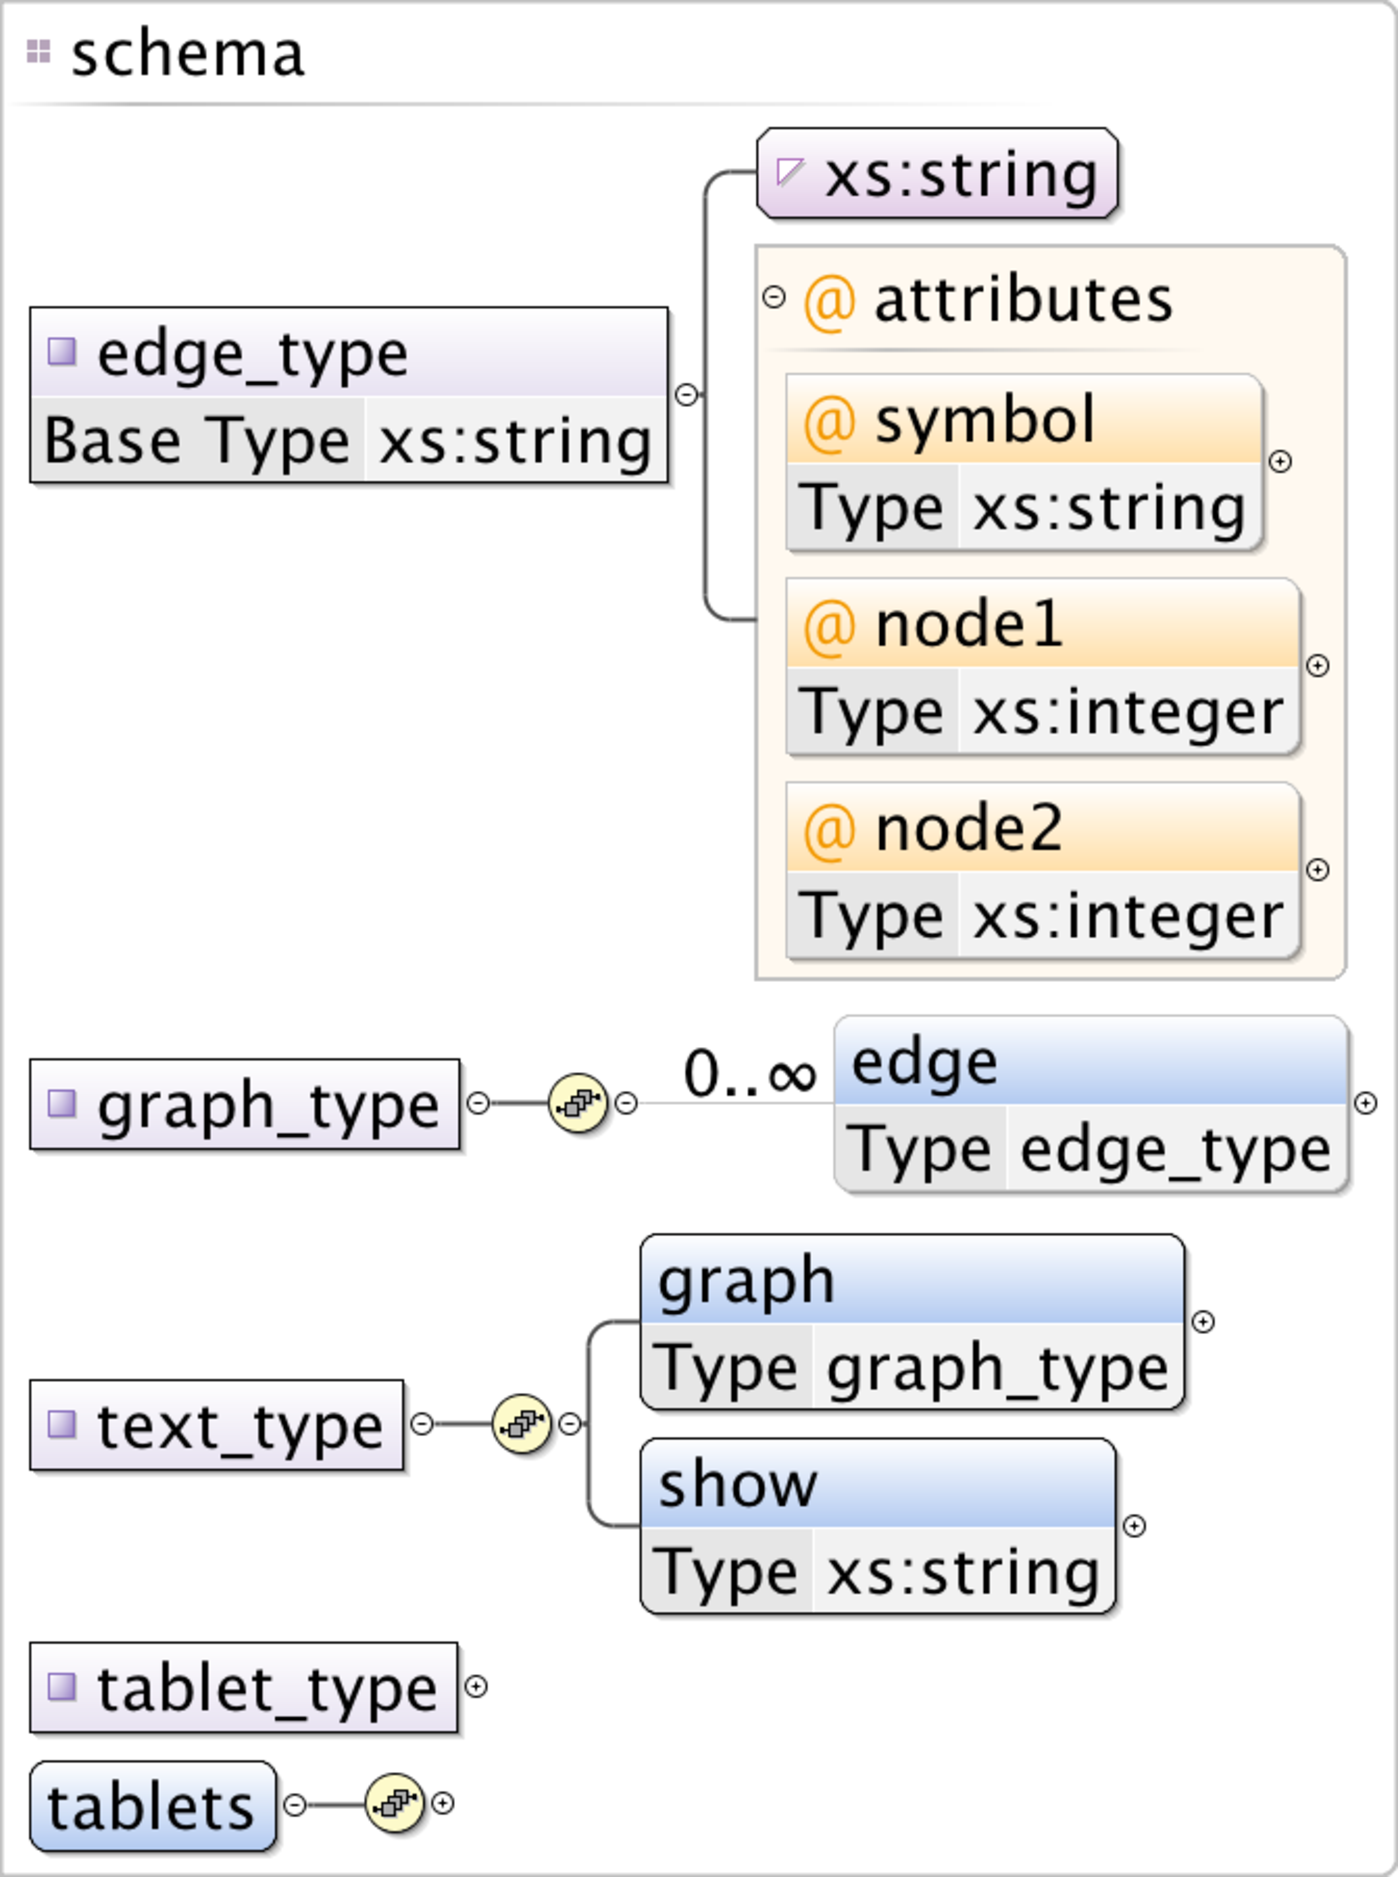
\includegraphics[width=120px]{../diagramy/schema_text.pdf}
 }
   \subfigure[element tablet]{
  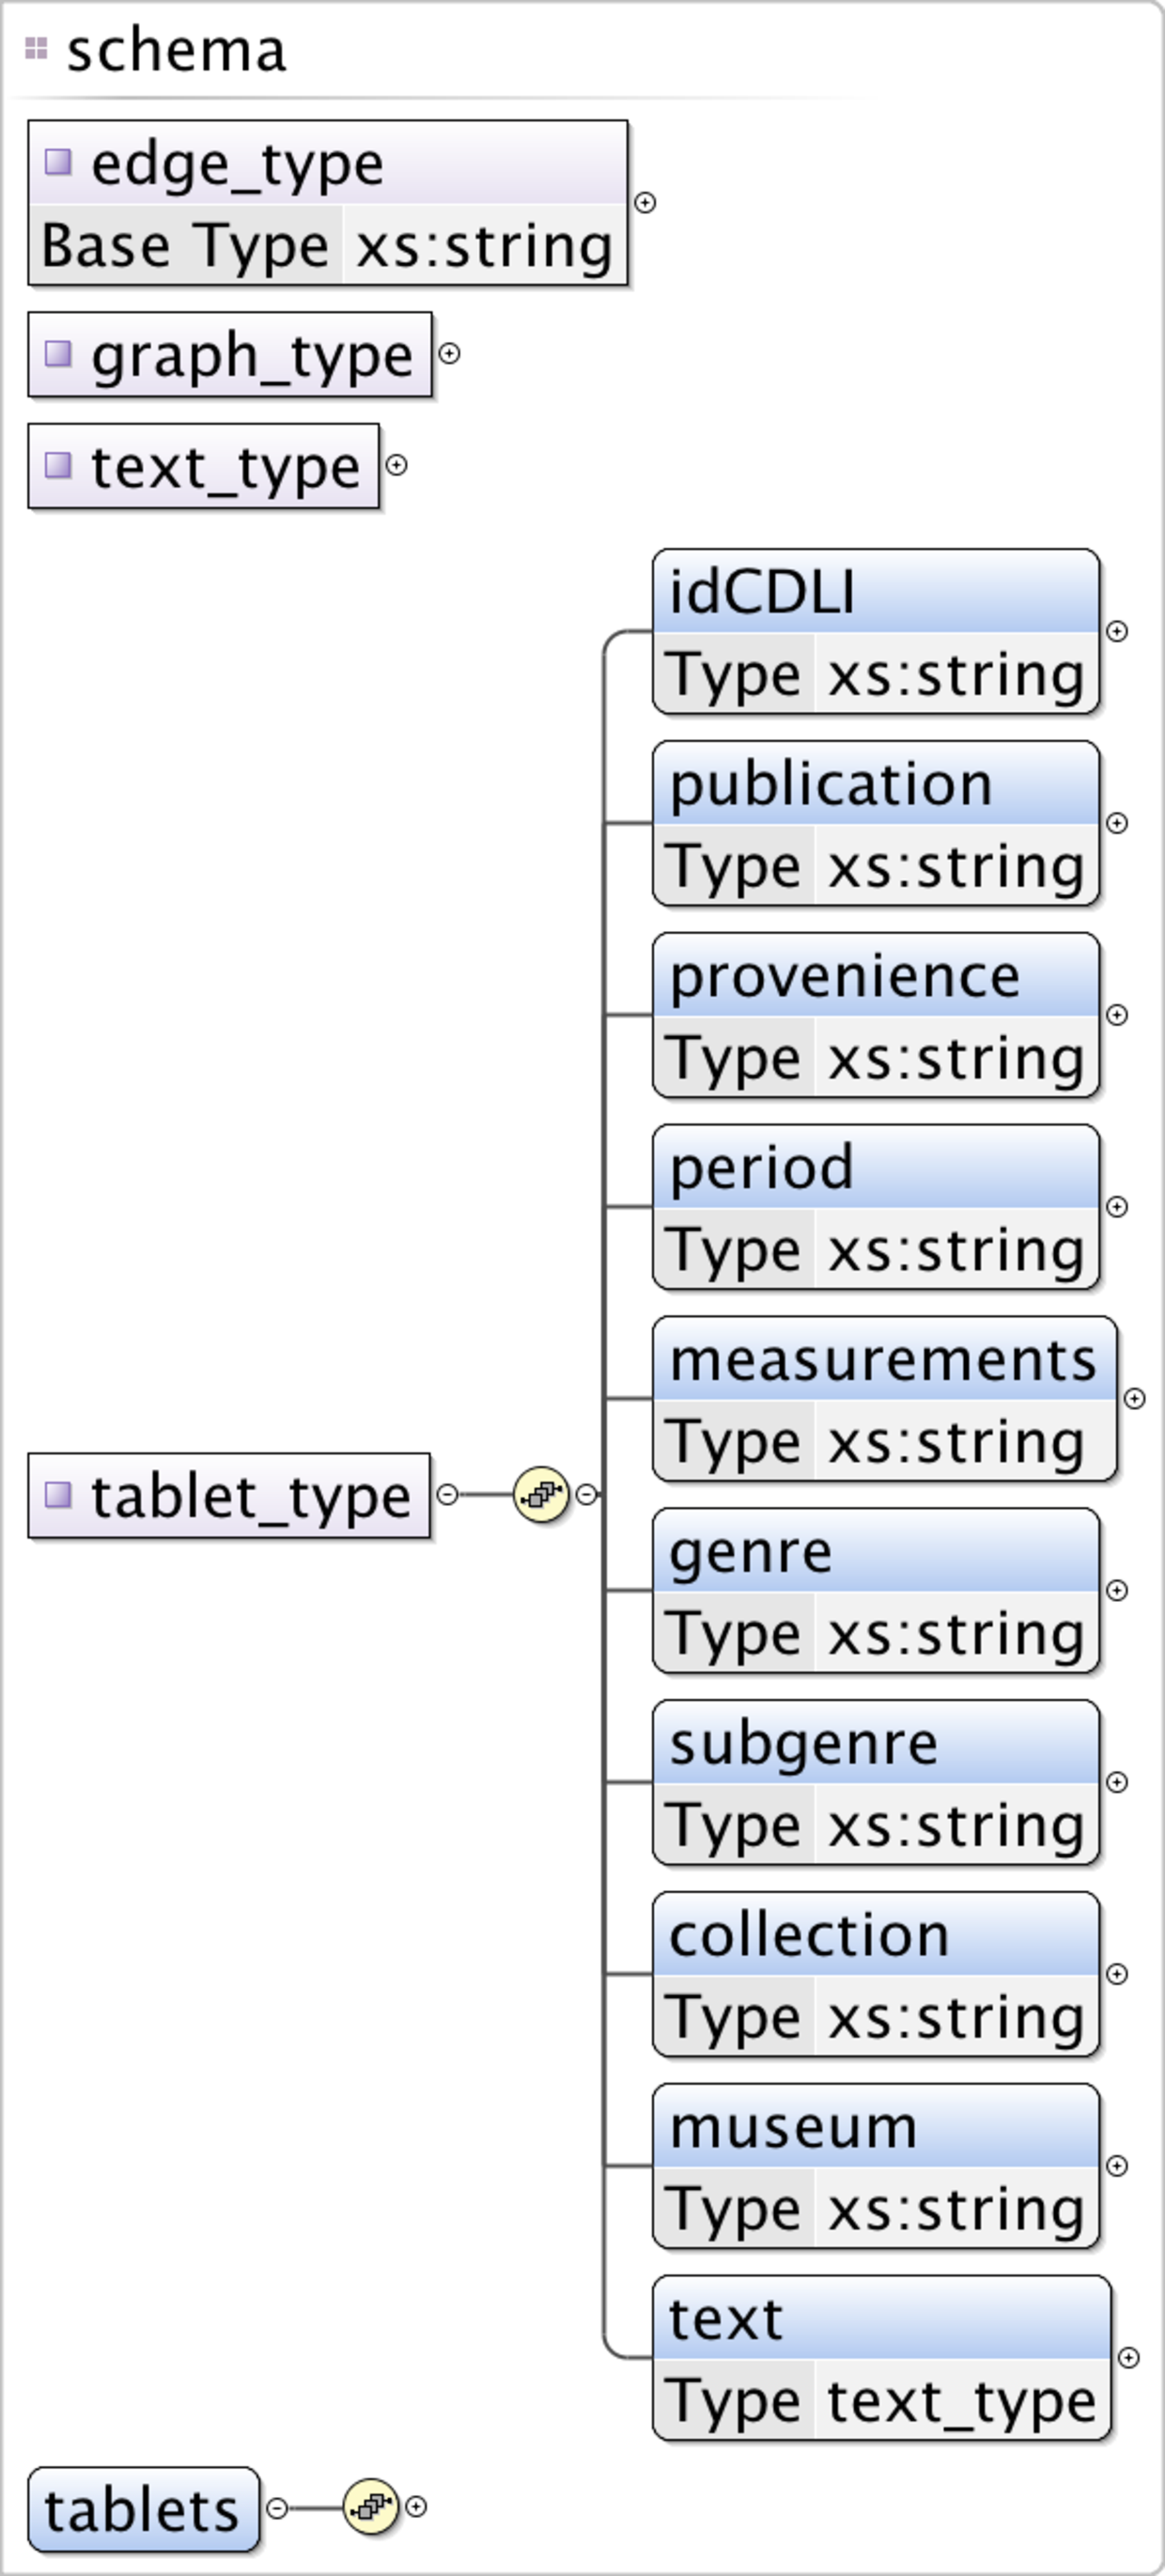
\includegraphics[width=120px]{../diagramy/schema_tablet.pdf}
 }
 \subfigure[element tablets]{
  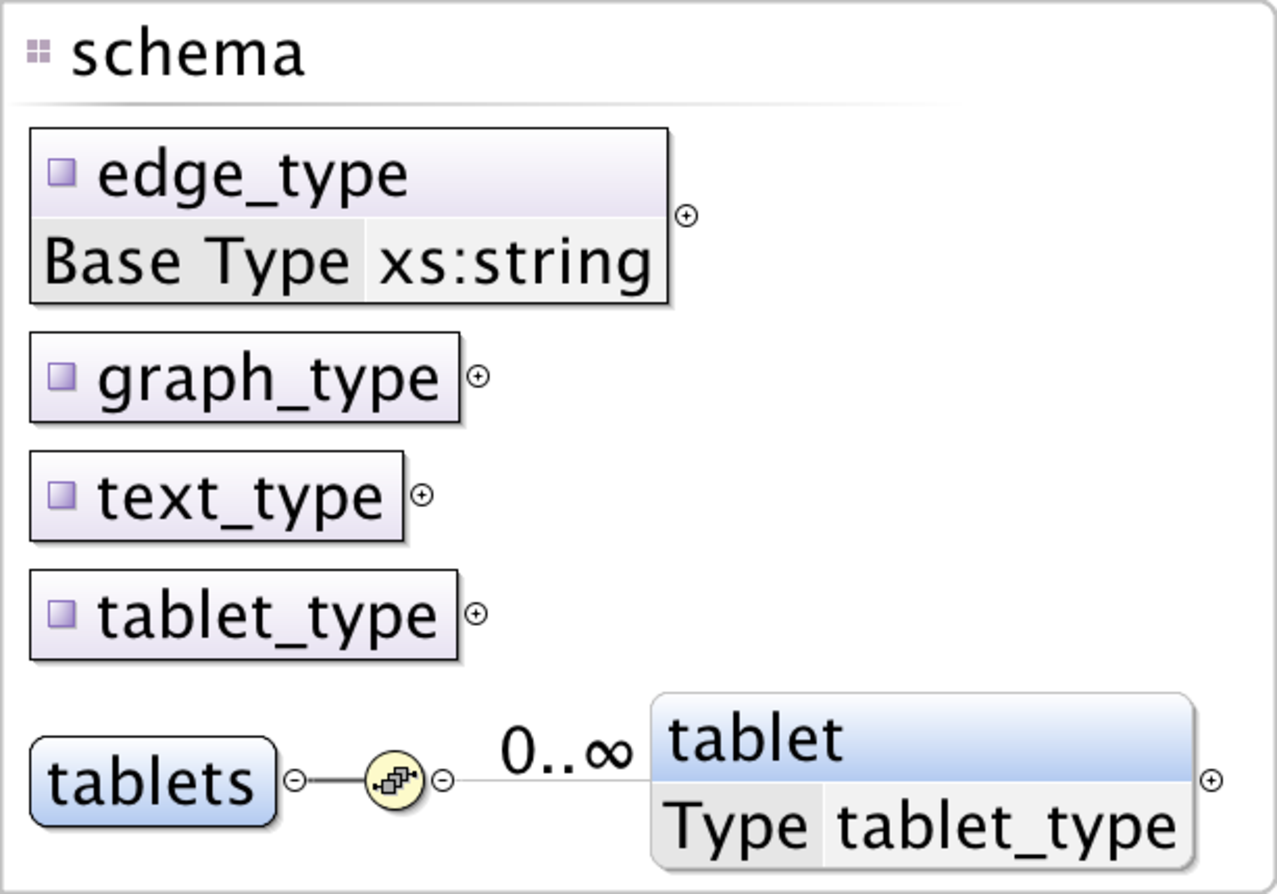
\includegraphics[width=120px]{../diagramy/schema_tablets.pdf}
 }
 \caption[Schematy poszczególnych elementów XML]{Schematy poszczególnych elementów XML\\ \footnotesize{kolor pomarańczowy oznacza atrybuty, a niebieski elementy}}
\end{figure}



Schemat dokumentu zamieszczony powyżej jest graficznym przedstawieniem dokumentu XML Schema (dodatek) 
wygenerowanym przez program Oxygen.

Jest on oparty, podobnie jak w bazie PostgreSQL, na pomyśle dra Wojciecha Jaworskiego, 
 aby przedstawić treść tabliczki w formie grafu. 
Każda krawędź tego grafu (odpowiadająca odczytowi) jest oddzielnym elementem, zawierającym atrybuty \textit{node1}, \textit{node2} 
i \textit{symbol}.
Atrybuty \textit{node1} oraz \textit{node2} oznaczają numery węzłów grafu,
natomiast atrybut \textit{symbol} to typ symbolu znajdującego się na danej krawędzi. 
Dodatkowo przechowujemy treść tabliczki w formie napisu (element \textit{show}). 

Metadane tabliczek przechowywane są w postaci podelementów elementu \textit{tablet}.


\subsubsection{Translator\_xml}
Do przeszukiwania dokumentu XML wykorzystywany jest język XQuery, będący częścią rekomendacji W3C dotyczącej XML.\\
Proste zapytanie TQL jest tłumaczone na pojedynczą konstrukcję FLWOR (For Let Where Order by Return).\\

\paragraph{Stałe fragmenty zapytania}
Każde zapytanie w części For zawiera:
	\begin{verbatim}
	FOR $tablet IN .//tablet
\end{verbatim}
a w części Return:
  \begin{verbatim}RETURN <tablet>
		{$tablet/idCDLI}
		{$tablet/publication}
		{$tablet/provenience}
		{$tablet/period}
		{$tablet/measurements}
		{$tablet/genre}
		{$tablet/subgenre}
		{$tablet/collection}
		{$tablet/museum}
		{$tablet/text/show}
		<seq>...</seq>
	</tablet>
\end{verbatim}
Zawartość elementu seq zależy od ilości sekwencji, po których wyszukujemy. 

\paragraph{Tłumaczenie zapytań o atrybuty tabliczki}

\begin{longtable}{|p{2.5in}|p{3.5in}|}
\hline
{\bf Konstrukcja} & {\bf Tłumaczenie na XQuery}\\
\hline
\endhead
provenience: wartosc & \begin{verbatim}fn:matches($tablet/provenience,'^wartosc$')\end{verbatim}
\\
\hline
publication: wartosc & \begin{verbatim}fn:matches($tablet/publication,'^wartosc$')\end{verbatim}
\\
\hline
period: wartosc & \begin{verbatim}fn:matches($tablet/period,'^wartosc$')\end{verbatim}
\\
\hline
genre: wartosc & \begin{verbatim}(fn:matches($tablet/genre,'^wartosc$')
or fn:matches($tablet/subgenre,'^wartosc$'))\end{verbatim}
\\
\hline
cdli\_id: wartosc & \begin{verbatim}fn:matches($tablet/idCDLI,'^wartosc$')\end{verbatim}
\\
\hline
\end{longtable}


\paragraph{Tłumaczenie zapytań o treść tabliczki}
Każda sekwencja, po której wyszukujemy, powoduje dodanie do zapytania następujących konstrukcji:
\begin{itemize}
\item{do części Let:}
\begin{verbatim}
let $seq <id_sekw> := (
	for $edge_end in $tablet//edge
	for $edge_start in $tablet//edge
	where (
		fn:matches($edge_start,'^<sekw[0]>$')
		and (
			some $edge1 in $tablet//edge[@node1=$edge_start/@node2]
satisfies (fn:matches($edge1,'^<sekw[1]>$')
and ... 
and fn:matches($edge_end,'^<sekw[dl_sekw-1]>$')))))
return <seq<id_sekw>> {$edge_start/@node1} {$edge_end/@node2} </seq<id_sekw>>
\end{verbatim}
\item{do części Where}
\begin{verbatim}
$seq<id_sekw>
\end{verbatim}
\item{do części Return w elemecie seq}
\begin{verbatim}
$seq<id_sekw>
\end{verbatim}
\end{itemize}




\paragraph{Tłumaczenie operatorów}
Poniższe tłumaczenia dotyczą zarówno konstrukcji prostych, jak i złożonych.

\begin{longtable}{|p{1in}|p{3in}|}
\hline
{\bf Operator} & {\bf Tłumaczenie}\\
\hline
\endhead
/ & \begin{verbatim}(<zapytanie1> or <zapytanie2>) \end{verbatim} \\
\hline
-- & \begin{verbatim}not (<zapytanie_negowane>) \end{verbatim}\\  
\hline
+ & \begin{verbatim}(<zapytanie1> and <zapytanie2>) \end{verbatim}\\ 
\hline
* & \begin{verbatim} .*\end{verbatim}  \\ 
\hline
\end{longtable}

\paragraph{Zapytania złożone}
Zapytanie złożone, składające się z wielu zapytań prostych tłumaczymy na sekwencję zapytań XQuery połączonych znakiem ','.

\subsubsection{Database\_xml}
Moduł \textit{Database\_xml} Odpowiada za wywołanie zapytania i zapisanie wyniku do struktury Tablets.
Jako bazę danych wykorzystujemy plik XML, określony w pliku konfiguracyjnym xml.conf. 
Do wyszukiwania wykorzystujemy procesor XQuery Zorba \cite{zorba}. 
Posiada on API m.in. do C++, które pozwala na przekazanie zapytania do bazy oraz przetworzenie wyniku.


%\chapter{Dokumentacja użytkowa i opis implementacji}\label{r:impl}
\chapter*{Podsumowanie}
\addcontentsline{toc}{chapter}{Podsumowanie}
\section*{Podsumowanie projektu}
\addcontentsline{toc}{section}{Podsumowanie projektu}
Przedstawiona w niniejszej pracy realizacja języka TQL spełnia najważniejsze postulaty. 
Po pierwsze jest on intuicyjny i prosty w użyciu dla osób znających jedynie dziedzinę problemu.
% (co potwierdza opinia dr hab. Marka Stępnia)
Po drugie minimalnie ogranicza siłę wyrazu, pozwalając na tworzenie skomplikowanych zapytań.

%ograniczenia: prezentacja wyników, zmiana danych
Język TQL ma jednak kilka ograniczeń w stosunku do typowych języków zapytań. 
Największym z nich jest brak wpływu na postać wyniku, co utrudnia np. zbieranie danych statystycznych 
(m.in. nie da się spytać o ilość tabliczek spełniających dane kryteria). 
Można jednak stworzyć narzędzia do samej prezentacji wyników zapytań, które pokonają to ograniczenie. 

Warto również zastanowić się nad możliwością sortowania wyników zapytań. W obecnej wersji TQL moża to zrobić na poziomie interfejsu, jednak
dodanie takiej funkcjonalności do języka pozwoliłoby na sortowanie bezpośrednio w bazie danych.

Należy pamiętać, że TQL jest jedynie językiem wyszukiwania -- w przeciwieństwie do wielu innych języków zapytań
nie udostępnia możliwości zmieniania danych znajdujących się w bazie, ani dodawania nowych. 

%ograniczenia: zapytanie którego się nie da wyrazić
Siła wyrazu języka TQL jest ograniczona w minimalnym stopniu.
Przykładem zapytania, którego nie sa się w nim wyrazić, jest
"znajdź tabliczki, które zawierają frazę zaczynającą się od słowa udu, której drugim słowem nie jest słowo ban".
Ogólnie TQL pozwala tworzyć zapytania w oparciu o frazy, określone w całości lub częściowo, ale nie pozwala konstruować warunków
dotyczących fragmentów fraz. Godzimy się na to ograniczenie, ponieważ najczęściej nie jest to potrzebne.
% Niemniej jednak
%warto rozważyć alternatywną konstrukcję języka, która umożliwi zapisywanie tego typu zapytań.





%zalety: wykorzystanie w innych dziedzinach
Dzięki specyficznym cechom języka TQL, można dostosować go do wykorzystania w innych dziedzinach. 
Należy tu wspomnieć o braku ograniczenia ilości i nazw pól, po których można wyszukiwać, oraz przystosowaniu 
do wyszukiwania wg kryteriów dotyczących danych tekstowych. 
Na podstawie TQL można łatwo stworzyć rodzinę języków dla różnych dziedzin zajmujących się przeszukiwaniem tekstów.

%zalety: łatwość implementacji
W ramach niniejszej pracy zaprezentowane zostały dwie implementacje języka TQL. 
Po stworzeniu pierwszej, czas potrzebny na drugą był już niewielki. 
Największym zadaniem było przetłumaczenie poszczególnych konstrukcji TQL na XQuery. 
Pozwala to sądzić, że każda kolejna implementacja, dla różnych typów baz i różnych schematów danych, 
nie będzie wymagała dużego nakładu pracy. 

\newpage 

\section*{Możliwości rozwoju}
\addcontentsline{toc}{section}{Możliwości rozwoju}
\begin{figure}[h]
 \centering
 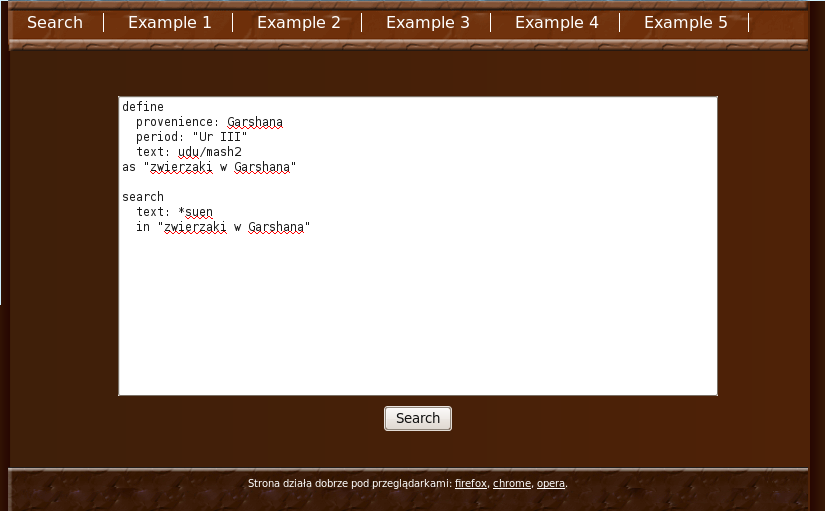
\includegraphics[width=450px]{../diagramy/wyszuk_zapyt.png}
 % wyszuk_zapyt.png: 811x524 pixel, 72dpi, 28.61x18.49 cm, bb=0 0 811 524
 \caption{Okno do wprowadzania zapytania}
 \label{fig:wyszuk_zapyt}
\end{figure}

\begin{figure}[h]
 \centering
 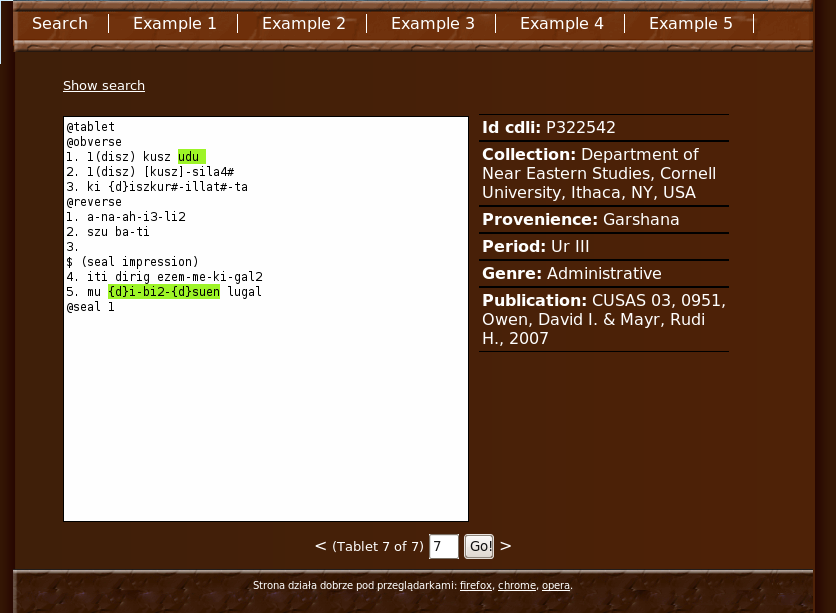
\includegraphics[width=450px]{../diagramy/wyszuk_wynik.png}
 % wyszuk_wynik.png: 823x628 pixel, 72dpi, 29.03x22.15 cm, bb=0 0 823 628
 \caption{Sposób prezentacji wyników zapytania}
 \label{fig:wyszuk_wynik}
\end{figure}

%co dalej
Jako dodatek do pracy stworzyłyśmy stronę internetową umożliwiającą zadanie zapytania w języku TQL i prezentującą wyniki. 
Jej wygląd jest przedstawiony na rysunkach \ref{fig:wyszuk_zapyt} oraz \ref{fig:wyszuk_wynik}.
% TODO: W chwili obecnej jest ona dostępna na stronie \url{http://students.mimuw.edu.pl/~/jw234694/sumlib/}.
Stanowi ona zalążek przyjaznego interfejsu użytkownika dla naukowców, którzy będą współpracować z TQL. Plany jej rozwoju
uwzględniają między innymi funkcjonalność graficznego budowanie zapytania.
% TODO: walnąć rozdzialik o graficznym bilderze
Na chwilę obecną serwis internetowy jest w trakcie udostępniania Wydziałowi Historii UW.
Jego pracownicy będą pierwszymi testerami całego rozwiązania.

Poza tym warto nawiązać współpracę z projektem CDLI, (zob. rozdział \ref{chapter:cdli}).
Implementacja TQL dla bazy CDLI, wraz z interfejsem WWW, z pewnością byłaby przydatnym narzędziem dla sumerologów na całym świecie.

W dalszej perspektywie można rozwinąć język TQL między innymi o wyszukiwanie wg klinów i wg tagów. 
Pierwsze z nich wymaga przetłumaczenia odczytów na kliny oraz umieszczenia tych informacji w bazie danych.
Drugie natomiast potrzebuje narzędzia do wykrywania poszczególnych tagów
(postaci, miar, dat, liczb itp) lub do ich zaznaczania przez sumerologów.

Dodatkowo warto stworzyć narzędzie do analizy uszkodzonych fragmentów i wykrywania błędów w odczytach tekstów. 
Dzięki niemu można by zmniejszyć ryzyko pominięcia istotnych tabliczek podczas wyszukiwania. 

Rozwój projektu będzie zależał również od potrzeb zgłaszanych przez samych sumerologów.


%\section*{Dyskusja}
%\addcontentsline{toc}{section}{Dyskusja}
% co można by inaczej (``Dyskusje'')

% konstrukcja języka


% implementacja
%Przedstawiona w pracy implementacja TQL jest tylko przykładowa. W szczególności można rozważyć optymalizacje w modułach zależnych od bazy
%danych, czyli wybór takiego sposobu budowania zapytania docelowego, który pozwoli jak najszybciej je wykonać. 
% c++, LL, Boost spirit
% wymyśleć inne zapytanie na ``NOT''
%W tym momencie implementacja zapytania zawierającego "-- --" (not) jest dla bazy PostgreSQL nieoptymalna.
%Polega ona na wyszukaniu wszystkich tabliczek, następnie wyszukaniu tabliczek zawierających niechcianą frazę, a potem odjęciu obu wyników.
%Można tutaj zaproponować algorytm, który będzie działał szybciej.

% co jest złego w typowej relacyjnej bazie danych
%Innym problemem, który również warto rozważyć przy implementacji TQL, jest wybór odpowiedniego sposobu reprezentacji danych. Szeroko rozpowszechnione
%bazy relacyjne nie są najlepszym rozwiązaniem, gdyż trudno w nich przeprowadzać operacje na tekstach. Potrzebna jest baza, która umożliwi jednocześnie szybki
%dostęp do całego tekstu, jak również szybkie wyszukiwanie fraz. Pomysł przedstawienia treści tabliczki za pomocą grafu pozwala na łatwe wyszukiwanie fraz oraz
%alternatywnych tłumaczeń, jednak bazy relacyjne nie są przystosowane do przechowywania takich struktur danych.

% przenośność między systemami operacyjnymi



%\part*{Dodatki}
%\addcontentsline{toc}{part}{Dodatki}
\begin{appendix}
% \appendixpage
\part*{Dodatki}
\addcontentsline{toc}{part}{Dodatki}

\chapter{Schemat bazy danych xml}
\label{appendix:xmlsch}

\chapter*{Dodatki}
\addcontentsline{toc}{chapter}{Dodatki}
\section*{Schemat bazy danych xml}
\label{appendix:xmlsch}
\begin{verbatim}
<?xml version="1.0"?>
<xs:schema xmlns:xs="http://www.w3.org/2001/XMLSchema">
<xs:complexType name="edge_type">
  <xs:simpleContent>
    <xs:extension base="xs:string">
      <xs:attribute name="symbol" type="xs:string"/>
      <xs:attribute name="node1" type="xs:integer"/>
      <xs:attribute name="node2" type="xs:integer"/>
    </xs:extension>
  </xs:simpleContent>
</xs:complexType>
<xs:complexType name="graph_type">
  <xs:sequence>
    <xs:element name="edge" minOccurs="0" maxOccurs="unbounded" type="edge_type"/>
  </xs:sequence>
</xs:complexType>
<xs:complexType name="text_type">
  <xs:sequence>
    <xs:element name="graph" type="graph_type"/>
    <xs:element name="show" type="xs:string"/>
  </xs:sequence>
</xs:complexType>
\end{verbatim}

\begin{verbatim}
<xs:complexType name="tablet_type">
  <xs:sequence>
    <xs:element name="idCDLI" type="xs:string"/>
    <xs:element name="publication" type="xs:string"/>
    <xs:element name="provenience" type="xs:string"/>
    <xs:element name="period" type="xs:string"/>
    <xs:element name="measurements" type="xs:string"/>
    <xs:element name="genre" type="xs:string"/>
    <xs:element name="subgenre" type="xs:string"/>
    <xs:element name="collection" type="xs:string"/>
    <xs:element name="museum" type="xs:string"/>	
    <xs:element name="text" type="text_type"/>		
  </xs:sequence>
</xs:complexType>
<xs:element name="tablets">
  <xs:complexType>
    <xs:sequence>
      <xs:element name="tablet" type="tablet_type" minOccurs="0" maxOccurs="unbounded"/>
    </xs:sequence>
  </xs:complexType>
</xs:element>
</xs:schema>
\end{verbatim}



\end{appendix}

\begin{thebibliography}{99}
\addcontentsline{toc}{chapter}{Bibliografia}
\bibitem{powalka} Agata Powałka, Marek Stępień, Jerzy Tyszkiewicz, \textit{Automatyczna analiza dokumentów sumeryjskich}, 
Czas i przestrzeń, \url{http://www.czasiprzestrzen.wuw.pl/?id=str,sumeryjskich,1,0}
% TODO - zmienić na artykuł?
\bibitem{jaworski} Wojciech Jaworski, \textit{Modelowanie tresci sumeryjskich tekstów gospodarczych z epoki Ur~III}, 
\url{http://nlp.ipipan.waw.pl/NLP-SEMINAR/071119.pdf}, 19 listopada 2007
\bibitem{kuckenburg} Martin Kuckenburg, \textit{Pierwsze słowo}, Państwowy Instytut Wydawniczy, Warszawa 2006, rozdział 8, 9
\bibitem{fowler} Martin Fowler, \textit{Domain Specific Languages}, % TODO: sprawdzić która strona itp.
%DSL - the good, the bad and the ugly
\bibitem{mernik} Marjan Mernik, Jan Heering, Anthony M. Sloane, \textit{When and How to Develop Domain-Specific Languages}
\bibitem{cdli} Cuneiform Digital Library Initiative, \url{http://cdli.ucla.edu}
\bibitem{etcsl} The Electronic Text Corpus of Sumerian Literature, \url{http://etcsl.orinst.ox.ac.uk/}
\bibitem{bnfc} BNF Converter, \url{http://www.ohloh.net/p/12800} %- Strona projektu BNFC
\bibitem{cexplode} C-explode, \url{http://maz-programmersdiary.blogspot.com/2008/09/c-explode.html}
\bibitem{postgres} PostgreSQL, \url{http://www.postgresql.org/}
\bibitem{xquery} XQuery, \url{http://www.w3.org/XML/Query/}
\bibitem{zorba} Zorba - procesor XQuery, \url{http://www.zorba-xquery.com/}


%\bibitem[Bea65]{beaman} Juliusz Beaman, \textit{Morbidity of the Jolly function}, Mathematica Absurdica, 117 (1965) 338--9.

\end{thebibliography}

\listoffigures
% \listoftables

\end{document}


%%% Local Variables:
%%% mode: latex
%%% TeX-master: t
%%% coding: latin-2
%%% End:
